\documentclass[twoside,11pt]{article}

% Use adjustwidth environment to exceed column width (see example table in text)
\usepackage{jmlr2e}

\usepackage{float}
\usepackage{color}
\usepackage[usenames,dvipsnames,svgnames,table]{xcolor}

\usepackage{lastpage,fancyhdr,graphicx}
\usepackage{epstopdf}

\usepackage{amsmath}
\usepackage{threeparttable}

\usepackage{booktabs}

%% Include all macros below 

\newcommand{\p}{\mbox{\,.}}
\newcommand{\fl}[1]{\left \lfloor #1 \right \rfloor}
\newcommand{\g}[1]{\color{gray} #1 \color{black}}
\newcommand{\B}{{\mathbb B}}
% \newcommand{\G}{{\mathbb G}}
\newcommand{\cG}{{\mathcal G}}
\newcommand{\cS}{{\mathcal S}}
\newcommand{\Rbb}{{\mathbb R}}
\newcommand{\N}{{\mathbb N}}
\newcommand{\C}{{\mathscr C}}
\newcommand{\Co}{{\overline{\mathscr C}}}
\newcommand{\R}{{\mathscr R}}
\newcommand{\m}{{\overline{m}}}
\newcommand{\ok}{{\overline{\kappa}}}
\newcommand{\s}[1]{{\overline{#1}}}
\newcommand{\mmid}{\;\middle|\;}
\newcommand{\hide}[1]{}
\newcommand{\tab}{\hspace*{5mm}}
\newcommand{\stack}[2]{\genfrac{}{}{0pt}{}{#1}{#2}}

\floatstyle{ruled}
\newfloat{pseudo}{h}{lop}
\floatname{pseudo}{Algorithm}

\newcommand{\pb}[1]{\textcolor{OliveGreen}{\small #1 \textsuperscript{[pb]} }}

% Heading arguments are {volume}{year}{pages}{submitted}{published}{author-full-names}

\jmlrheading{1}{2000}{1-48}{12/16}{10/00}{Peter Bloem and Steven de Rooij}

% Short headings should be running head and authors last names

\ShortHeadings{Finding Network Motifs in Large Graphs}{Bloem and de Rooij}
\firstpageno{1}


\begin{document}

\title{Finding Network Motifs in Large Graphs using Compression as a Measure of Relevance}

\author{\name Peter Bloem \email vu@peterbloem.nl \\
       \addr Knowledge Representation and Reasoning Group\\
        VU University Amsterdam \\
		De Boelelaan 1105, 1081 HV Amsterdam, NL \AND
       \name Steven de Rooij \email steven.de.rooij@gmail.com \\
       \addr Mathematical Institute \\
        University of Leiden\\
        Niels Bohrweg 1, 2333 CA Leiden, NL}

\editor{\ldots}

\maketitle

\begin{abstract}%
We introduce a new method for finding \emph{network motifs}: interesting or informative subgraph patterns in a network. Subgraphs are motifs when their frequency in the data is high compared to the expected frequency under a \emph{null model}. To compute this expectation, a full or approximate count of the occurrences of a motif is normally repeated on as many as 1000 random graphs sampled from the null model; a prohibitively expensive step. We use ideas from the Minimum Description Length (MDL) literature to define a new measure of motif relevance. With our method, samples from the null model are not required. Instead we compute the probability of the data under the null model and compare this to the probability under a specially designed alternative model. With this new relevance test, we can search for motifs by random sampling, rather than requiring an accurate count of all instances of a motif. This allows motif analysis to scale to networks with billions of links, while still resulting in informative motifs. 
\end{abstract}

 \begin{keywords} graphs, minimum description length, unsupervised learning, pattern mining, network motifs \end{keywords}

\section{Introduction}

Graphlets are small, induced subgraphs a large network. \emph{Network motifs} \citep{milo2002network} are those graphlets that occur more frequently in the data than expected. Graphlets and network motifs are used for many purposes, for instance: as features in machine learning \citep{shervashidze2009efficient,wu2011characterizing}, as candidates for ``functional units'' of the system represented by the graph \citep{milo2002network}, as a method to reduce the complexity of the graph \citep{koutra2015summarizing} or as a building block in community detection \citep{arenas2008motif}. To be able to conclude that such frequent subgraphs really represent meaningful aspects of the data, we must first show that they are not simply a product of chance. That is, a subgraph may simply be a frequent subgraph in \emph{any} random graph: a subgraph is only a \emph{motif} if its frequency is higher \emph{than expected}.

This expectation is defined in reference to a \emph{null model}: a probability distribution over graphs. We determine what the expected frequency of the subgraph is under the null model, and if the observed frequency is substantially higher than this expectation, the subgraph is a motif.\footnotemark 

\footnotetext{Commonly, all possible graphlets of a given size are checked. Depending on the task, the full list of motif scores is used as a feature vector representing the graph, or the top-$k$ motifs are used by a domain expert as candidates for further analysis. Since each motif is judged by a hypothesis test, the reader may wonder whether this approach constitutes multiple testing. However, as discussed in Section~\ref{section:multiple-testing}, motif analysis uses the significance test merely as a pattern-mining heuristic, not as a true statistical test.} 

Unfortunately, there is usually no efficient way to compute the expected frequency of a subgraph under a null model. The most common approach is to generate a large number of random graphs, say 1000, from the null model and compare the frequencies of the subgraph in the graphs in this sample to its frequency in the data \citep{milo2002network}. This means that any resources invested in extracting the motifs from the data must be invested again 1000 times to find out which subgraphs are motifs.

We introduce an alternative method that does not require such sampling from the null model. To achieve this, we use two probability distributions on graphs: the null model $p^\text{null}$, and a distribution $p^\text{motif}$ under which graphs with one or more frequent subgraphs have high probability. If a subgraph $M$ of a given graph $G$ allows us to show that $p^\text{motif}(G)$ is larger than $p^\text{null}(G)$, then $M$ is a motif. 

To design $p^\text{motif}$, we use the Minimum Description Length (MDL) Principle \citep{rissanen1978modeling,grunwald2007minimum}. We design a description method for graphs, a \emph{code}, which uses the frequent occurrence of a potential motif $M$ to create a compressed description of the graph. Our approach is analogous to compressing text by giving a frequent word a brief codeword: we describe $M$ once and refer back to this description wherever it occurs. 

By a commonly used correspondence between codes and probability distributions (detailed in the preliminaries), we derive $p^\text{motif}$ from this code, a distribution that assigns high probability to graphs containing motifs. Section~\ref{section:model-selection} explains the principle and its theoretical justification.

This approach removes the need to take samples from the null model: we only need to compute $p^\text{null}(G)$ and $p^\text{motif}(G)$. It also removes the need for accurate subgraph counts. For a potential motif $M$, we only need to find enough occurrences in  $G$ to achieve the required level of compression. We use a simple random sampling algorithm, which operates in constant time with respect to the size of the graph. These two improvements lead to a considerable increase in the scale of graphs which can be analysed. 

Specifically, we show the following:
\begin{itemize}
  \item On commodity hardware, our method can be used to analyze graphs with millions of links in minutes. We can analyze graphs with billions of links in under 9 hours on a basic compute node, and in about 45 hours on hardware equivalent to a single laptop (Section~\ref{section:large}). Contrast this with the current scale of motif analysis, which is limited to graphs in the order of 1000 to 10 000 links.\footnote{\citet{hovcevar2014combinatorial} report a complete subgraph \emph{count} on a graph with 137 775 links, the largest we have found, but the comparison to a null model required for motif analysis is not performed.}
  \item The method can be used for motifs with at least 10 nodes, although space and time complexity do increase for larger motif sizes (Section~\ref{section:large}).  
  \item Our method can retrieve motifs that have been injected into the data, even at relatively low quantities (Section~\ref{section:recovering}).
  \item In real data, the judgments on whether a subgraph is a motif or not produced by our method are as informative in characterizing the graph as those returned by the traditional method. We evaluate this by using the motif judgments as binary features in a graph classification task (Section~\ref{section:classification}). 
\end{itemize}

The paper is structured as follows. The next two subsections discuss related work and preliminary information on graphs and MDL. Section~\ref{section:model-selection} provides an in-depth explanation of the method we use to perform hypothesis testing through MDL. In Section~\ref{section:motif-code}, we detail our motif model. In Section~\ref{section:null-models} we detail the three null-models we will use to test its performance. In Section \ref{section:experiments}, we detail briefly how we search for motifs, and select candidates, and then report the results of four experiments to validate the claims made above.

All software used in this paper is available open source. \footnote{See \url{https://github.com/pbloem/motive} and \url{https://github.com/pbloem/motive-cls}.} 

\subsection{Related Work}
Many different algorithms, techniques and tools have been proposed for the detection of motifs, all based on a common framework, consisting of three basic steps:

\begin{enumerate}
  \item Obtain a count $f_M$ of the frequency of subgraph $M$ in graph $G$. \label{step1}
  \item Obtain or approximate the probability distribution over the number of instances $F_M$ given that $G$ came from a particular null model $p^\text{null}$.  \label{step2}
  \item If $p^\text{null}(F_M \leq f_M) \leq \alpha$ (usually with $\alpha = 0.05$), we consider $M$ a motif. \label{step3}
\end{enumerate} 

\noindent This was the approach proposed by \cite{milo2002network}, in the paper that where the phrase \emph{network motif} was coined. One problem with this approach is that it is very expensive to perform naively. Step \ref{step1} requires a full \emph{graph census},\footnote{A graph census for size $k$ counts, for each connected graph $M$ of size $k$, the number of times the graph occurs as an induced subgraph of the data.} and since the probability in step \ref{step3} cannot usually be computed analytically, we are required to perform the census again on thousands of graphs sampled from the null model in order to approximate it. 

Most subsequent approaches have attempted to improve efficiency by focusing on step~\ref{step1}: either by designing algorithms to get exact counts more efficiently \citep{koskas2011nemo,li2012netmode,khakabimamaghani2013quatexelero,meira2014acc}, or by approximating the exact count. The most extreme example of the latter is \citet{kashtan2004efficient}, which simply counts randomly sampled subgraphs. The complexity of this algorithm is \emph{independent of the size of the data}, suggesting an exceptionally scalable approach to motif detection. Unfortunately, while the resulting ranking of motifs by frequency is usually accurate, the estimate of their total frequency is not \citep{wernicke2005faster}, which makes it difficult to build on this approach in steps \ref{step2} and \ref{step3}. Other algorithms provide more accurate and unbiased estimates \citep{wernicke2005faster,ribeiro2010g,bhuiyan2012guise,jha2015path,slota2014complex,paredes2015rand}, but they do not maintain the extreme scalability of the sampling approach.

We take an alternative route: instead of improving the sampling, we change the measure of motif relevance: we define a new hypothesis test as an alternative to steps \ref{step2} and \ref{step3}, which does not require an accurate estimate of the number of instances of the motif. All that is required is a set of some instances; as many as can be found with the resources available. This means that the highly scalable sampling approach from \cite{kashtan2004efficient} can be maintained.

The frequency of a motif is not the only statistic we can use. We might, for instance, compare the level of clustering among the instances with the value expected under the null model. This is relevant, because our compression method can be seen as a combination of several statistics. Specifically, properties that allow a motif to reject the null hypothesis are: a high frequency of \emph{non-overlapping}\footnotemark~instances, a large number of instances with few links to nodes outside the instance and a high number of internal links. While this deviates from the more common statistic of pure frequency, we believe these are all properties that fit the intuitive idea of a motif. In the graph mining literature, different notions of frequency of a subgraph are often called \emph{support measures} \citep{wang2012efficiently}. 

\footnotetext{Using non-overlapping instances is known as \emph{frequency concept 3} in \citep{schreiber2004towards}.}

\cite{picard2008assessing} provide an analytical solution, which can perform the hypothesis test without generating a random sample of networks. The constraint here is that the null model should be \emph{exchangeable}. For the commonly used degree-sequence model, a sampling based-approximation is used.\footnotemark~The complexity of the hypothesis test is independent of the the size of the graph, but it is is $O(k!^2)$ in the size $k$ of the motif. While this method could be used for very scalable motif detection (for small $k$, with exchangeable null models), we are not aware of any practical efforts to this effect.

\footnotetext{The degree sequence model always seems to require approximate solutions. FANMOD \citep{wernicke2005faster} requires the computation of the number of graphs with a given degree sequence and a specific subgraph at a particular location. They use the approximation from \citet{bender1978asymptotic}, which is asymptotically correct, but provides no bouds for the case of a finite graph. For our algorithm, we require a similar estimate (the number of graphs with a particular degree sequence). We use the sampling-based methods from \cite{blitzstein2011sequential,charo2010efficient}. These are slower, but they provide a clearer bound on the accuracy of the estimate, as described in Section~\ref{section:null models} and the supplementary materials.}

The idea that compression can be used as a heuristic for subgraph discovery was also used in the SUBDUE algorithm by \citet{cook1994substructure}. Our approach uses a more refined compression method and we connect it explicitly to the framework of motif analysis and the use of hypothesis tests as a heuristic for pattern mining. We also exploit the possibility that the MDL approach offers, for a very scalable sampling algorithm, to replace the more restrictive beamsearch used in SUBDUE. In itemset mining, the use of MDL has a long and successful history, as detailed by \citet[Chapter~8]{aggarwal2014frequent}.

The literature behind graph mining, graphlets and network motifs seems to have developed largely in parallel, repeating much of the same ground. While graph mining tends to focus on datasets consisting of many small graphs, rather than one large graph, there are efforts focusing on the latter. For a good overview of recent work, we refer the reader to \citet[Chapter~13]{aggarwal2014frequent}. Research on graphlets likewise tends to focus on datasets where each instance is represented by a separate graph, usually in a classification setting \cite{shervashidze2009efficient}. However, recently, a great deal of machine learning research has emerged that deals with the case where the dataset consists of a single graph, and the instances to be classified are a subset of its nodes \citep{pham2016column}. Where graphlet approaches tend to focus on the raw frequencies of subgraphs in the data, network motif research focuses on the frequency relative to the expectation under a null model.  

\subsection{Preliminaries: Graphs and Codes}
\label{section:preliminaries}

\paragraph{Graphs} A graph $G$ of size $n$ is a tuple $(V_G, E_G)$ containing a set of \emph{nodes} (or \emph{vertices}) $V_G$ and a set of \emph{links} (or \emph{edges}) $E_G$. For convenience in defining probability distributions on graphs, $V_G$ is always the set of the first $n$ natural numbers. $E_G$ contains pairs of elements from $V_G$. For the dimensions of the graph, we use the functions $n(G) = |V_G|$ and $m(G) = |E_G|$. If a graph $G$ is \emph{directed}, the pairs in $E_G$ are ordered, if it is \emph{undirected}, they are unordered. A \emph{multigraph} has the same definition as a graph, but with $E_G$ a multiset, i.e. the same link can occur more than once.

There are many types of graphs and tailoring a method to each one is a laborious task. Here, we limit ourselves to datasets that are (directed or undirected) \emph{simple graphs}: i.e. no link connects a node to itself and the same link cannot occur more than once. Probability distributions on the set of simple graphs are usually the most complex, so that we can trust that a method that works for simple graphs is easily translated to other types.

Two graphs $G$ and $H$ are \emph{isomorphic} if there exists a bijection $f: N_G \to N_H$ on the nodes of $G$ such that two nodes $a$ and $b$ are adjacent in $G$ if and only if $f(a)$ and $f(b)$ are adjacent in $H$. If two graphs $G$ and $H$ are isomorphic, we say that they belong to the same \emph{isomorphism class} $[G]$.

\paragraph{Codes and MDL} The intuition behind MDL is that compressing data and learning from it are much the same process: in both cases, we are analyzing data to find patterns that are characteristic for the data, or patterns that represent the data well. This is not just an intuition, there exists a very precise correspondence between optimizing for probability and optimizing for description length. We will detail the basic principle below, and give an intuitive example of how we apply the method in the next section. For more details, we refer the reader to \cite{grunwald2007minimum}.
 
Let $\B$ be the set of all finite-length binary strings. We use $|b|$ to represent the length of $b \in \B$. Let $\log(x) = \log_2(x)$. A \emph{code} for a set of objects $\cal X$ (usually graphs, in our case) is an injective function $f: {\cal X} \to \B$, mapping objects to binary code words. All codes in this paper are \emph{prefix-free}: no code word is the prefix of another. We will denote a \emph{codelength function} with the letter $L$, ie. $L(x) = |f(x)|$. It is common practice to compute $L$ directly, without explicitly computing the codewords. In fact, we will adopt the convention of referring to $L$ itself as a code.

A well known result in information theory is the association between codes and probability distributions, implied by the  \emph{Kraft inequality}: for each probability distribution $p$ on $\cal X$, there exists a prefix-free code $L$ such that for all $x \in \cal X$: $- \log p(x) \leq L(x) < -\log p(x) + 1$. Inversely, for every prefix-free code $L$ for $\cal X$, there exists a probability distribution $p$ such that for all $x \in \cal X$: $p(x) = 2^{-L(x)}$. For proofs, see \cite[Section~3.2.1]{grunwald2007minimum} or \cite[Theorem~5.2.1]{cover2006elements}. To explain the intuition, note that we can easily transform a code $L$ into a sampling algorithm for $p$ by feeding the decoding function random bits until it produces an output. To transform a probability distribution to a code, techniques like arithmetic coding \citep{rissanen1979arithmetic} can be used. 

As explained by \citet[page 96]{grunwald2007minimum}, the fact that $-\log p^*(x)$ is real-valued and $L^*(x)$ is integer-valued can be safely ignored and we may \emph{identify} codes with probability distributions, allowing codes to take non-integer values. 

When we need to encode a single choice from a finite set $S$ of options, we will often use the code with length $\log |S|$, corresponding to a uniform distribution on $S$. In some cases, we can allow codes with multiple codewords for a single object. If a code $L$ has multiple codewords for some object  $x$, we may indicate the choice for a particular codeword by a parameter $a$ as $L(x; a)$.

\section{Model Rejection by Codelength}

\label{section:model-selection}

In this section we provide an intuitive discussion of the principle behind our method. To simplify the explanation, we will illustrate the idea on a simpler problem than motif analysis: determining whether a single large clique in a graph is an unusual feature, or to be expected under a particular null model. For certain null models, such as the Erd\H{o}s-Renyi (ER) model, the expected size of the largest clique is well understood \citep{bollobas1976cliques}. For other models, less so. Without resorting to sampling a large number of graphs from the model, how can we determine that a particular size of clique is unusually large under a given null model? We will define two codes, $L^\text{null}$ and $L^\text{clique}$, and show that if $L^\text{clique}$ compresses the data better than $L^\text{null}$ by enough bits, it is very unlikely that the data came from the null model, and we cannot dismiss the clique as a consequence of random chance.

Consider an undirected graph $G$ containing a large clique: all nodes in some subset $V_C \subseteq V_G$ are directly connected to one another. We can describe the graph by first describing the set $V_C$, and then describing $G$ in a canonical manner. Since every node in $V_C$ is connected to every other node in the clique, we can omit these links from the second part of our description, shortening the total description length, if $V_C$ is large enough. This gives us a code $L^\text{clique}$ with short codelengths for graphs containing a single large clique, and---by the correspondence mentioned in the preliminaries---also a probability distribution $p^\text{clique}$ with high probabilities for graphs with a large clique. The principle is illustrated in Figure~\ref{figure:clique-example}.

It is important to be aware that this is a code with \emph{multiple codewords for the same graph}. To convert this to a probability distribution, we sum the probabilities of all codewords: $p^\text{clique}(G) = \sum_c 2^{-L^\text{clique}(G;c)}$, where each $c$ identifies a clique in $G$.\footnote{We can convert $p^\text{clique}$ back to a another code by taking the negative logarithm: $\bar L^\text{clique}(G) = -\log(G)$. $\bar L^\text{clique}$ is a superior code (it always lowerbounds $L^\text{clique}$), but inefficient to compute.} As we shall see, we can use such codes without problems, \emph{so long as they are not used as the null model}. For null models we require a code with a single codeword per graph.

Of course, there is no guarantee that of all the distributions with a bias towards large cliques, $p^\text{clique}$ is the precise distribution from which we sampled our data. Luckily, it does not need to be: as long as we can show that our clique-based model encodes the data more efficiently than the null model, the presence of the clique disproves the hypothesis that the data came from the null model. We do not know where it came from, but it did not come from the null model. Under the hypothesis that the null model was the source of the data, we can show that the probability that any other model compresses the data better by $k$ bits or more, decays exponentially in $k$. This is known as  the \emph{no-hypercompression inequality} \cite[p103]{grunwald2007minimum}. More precisely, let $p^\text{null}(x)$ be any probability distribution, with $L^\text{null}(x) = - \log p^\text{null}(x)$ and let $L(x)$ be \emph{any} code, then we have
\[
p^\text{null}\left(L^\text{null}(x) - L(x) \geq k\right) \leq 2^{-k} \p
\]

To provide some intuition for why this should be so, imagine that $L^\text{null}$ and $L$ are both codes from uniform distributions: $L^\text{null}$ provides each graph in $X^\text{null}$ with a codeword of constant length $n$, and $L$ provides each graph in $X$ with a codeword of constant length $n-k$. Then, $L^\text{null}$ provides enough codewords for $2^n$ graphs and, $L$ provides enough codewords for $2^{n-k}$ graphs. Thus, if a graph can be represented by both (and thus compressed by $k$ bits), its probability under the null model is at most $2^{-k}$. This is the basic principle allowing us to use compression for statistical purposes: \emph{there are exponentially fewer short codes than long ones, so compressible data is rare}.

To give a sense of scale; under the null model, the probability that $L^\text{clique}$ will compress the data better than the null model by 10 bits or more is less than one in one-thousand. For twenty bits, we get one in a million, for thirty bits, one in a billion, and so on. 

We can interpret this procedure as a hypothesis test: the difference in compression $\Delta$ between the null model and the alternative model is a statistic \cite[Example~14.2]{grunwald2007minimum}. The no-hypercompression inequality gives us a bound on the probability $p^\text{null}(D \geq k)$. To reject the null model with significance level $\alpha$, we must find some code on the set of all graphs and show that it compresses the data better than the null model by $k$ bits, with $2^{-k} \leq \alpha$. Any code will do, as long as it was chosen before seeing the data. The better we design our code, the greater the power of the test.

Note that $\Delta$ is also the logarithm of the likelihood ratio between the null model and $L$, so we can see this as a likelihood ratio test. We can also interpret the difference in codelength between two models $p_a$ and $p_b$  as the logarithm of the \emph{Bayes factor} $p_a(x)/p_b(x)$ \cite[Section~14.2.3]{grunwald2007minimum}. 

Now, while our test  \emph{rejects} the null model, it does not necessarily \emph{confirm} anything about the pattern we used to compress the data. We would like to make it as likely as possible that it was the pattern we are interested in (e.g. the clique) that allowed us to reject the null model, and not some other aspect of the alternative model. This is a complex problem and, it is difficult to provide any guarantees. If the alternative model stores, say, the linkset of a graph more efficiently than the null model does, it may well be that the alternative model always beats the null model, regardless of the pattern used. To rule out most such artifacts, we must re-use the same model we used for the null model within the alternative model to store every part of the graph except the pattern. There is usually an intuitive way to do this: for instance, in the alternative model for the clique, we store the graph in two parts: first the nodes belonging to the clique, and then the full graph, minus any links in the clique. If we use, say, the Erd\H{o}s-Renyi model as our null model, we also use it to store the graph in this second part of the code. In this way, we know that any compression achieved must be due to the clique.\footnotemark 

\footnotetext{The lack of guarantees may be a cause for skepticism. Consider, however, that the hypothesis test by itself  is \emph{never} proof that the pattern found is meaningful, only that the null hypothesis is incorrect. See also Section~\ref{section:multiple-testing}.}

\begin{figure}[tb]
  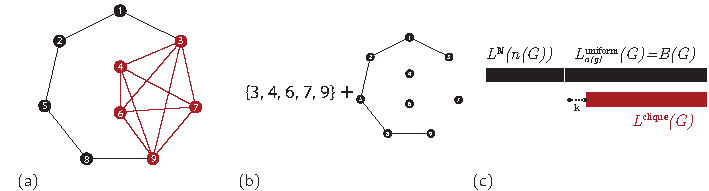
\includegraphics[width=\textwidth]{./images/mdlexplanation.pdf}
  \caption{A simple example of graph analysis by MDL: finding cliques. (a) The data. (b) A representation of the data that exploits the existence of a large clique. We first store a set indicating which nodes belong to the clique. We then store the graph, omitting those links that belong to the clique. (c) An illustration of the principle of a bound. For a complete code on graphs, using $L^{\text{uniform}}$, we need to first store the size of the graph using some arbitrary code on the integers $L^\N$. To make sure that it does not matter which code we choose for $L^\N$, we require our code ($L^{\text{clique}}$) to beat the bound $B(G)$ (by at least $k$ bits). }
   \label{figure:clique-example}
\end{figure}  

To ensure this, we aim to have the alternative model exploit only the pattern, and nothing else: we reuse the same model we used as the null model to store all of the graph, save for the pattern. For instance, in the example above, the clique model must store the graph minus the links of the clique. If we use the null model for this, we know that the only change between the null model and the alternative is the use of the clique, so that must be what made the difference. 

\subsection{Rejecting Multiple Null Models}

\label{section:multiplerejection}

A final benefit of this method is that we can reject multiple null models with a single test. In many situations we will have a function $B(G)$ that lowerbounds any code in some set $\cal L$. If our alternative model provides a codelength below $B(G) - k_\alpha$ with $k_\alpha$ the number of bits required for our chosen $\alpha$, we can reject all of $\cal L$.

As an example, Let $\cG_n$ be the set of all undirected graphs of size $n$. For our null model, we define a uniform code on such graphs: $L^\text{uniform}_n = \log |\cG_n|$. This null model captures the idea that the size of the graph is the only informative statistic: given the size, all graphs  are equally likely. However, it is \emph{parametrized}. It is currently not a code on \emph{all} graphs, just those of size $n$. To turn it into a code that can represent all graphs, we need to encode the parameter $n$ as well, with some code $L^\N$ over the natural numbers
\[
L^\text{complete}(G) = L^\N(n(G)) + L^\text{uniform}_{n(G)}(G) \p
\]
This is called \emph{two-part coding}, we encode the parameters of a model first, and then the data given the parameters. For some parametrized model $L_\theta$, we can choose any code for $\theta$ to make it complete. We will call the set of all such complete codes the \emph{two-part codes on $L_\theta$}. Note that we can simply concatenate the two codewords, since all codes are prefix-free.

Which code we choose for the parameter is arbitrary. We may be able to reject the uniform code for one choice of $L^\N$, or several, but how can we prove that $L^\text{complete}$ will be rejected whatever $L^\N$ we choose? Instead of choosing an arbitrary code for the size, we can use the \emph{bound} $B(G) = L^\text{uniform}_{n(G)}(G)$ as our null model. This is not a code, but it \emph{is} a lower bound for any two-part code on $L^\text{uniform}_n$. If $L^\text{clique}(G)$ is shorter than $B(G)$, it is also shorter than $L^\text{complete}(G)$ whatever the choice of $L^\N$.\footnotemark

\footnotetext{
In probabilistic terms, the code on the parameter corresponds to a prior on the parameter. The two-part codes correspond to maximum likelihood posterior probabilities: $p(\hat\theta) p(x \mid\hat\theta)$. Our bound corresponds to the maximal likelihood of the data: $p(x \mid \hat \theta)$. This shows us that the bound applies not only to the two-part codes, but also to the full Bayesian mixture: $\sum_\theta p(x \mid \theta) p(\theta) \leq \sum_\theta p(x \mid \hat\theta) p(\theta) = p(x \mid\hat\theta)$
} 

% Contrast this with the traditional approach, where we would define a statistic on $G$, like the size of the largest clique, and compare the observed value of the statistic with the expectation under the null model. In this case the models would have to be rejected with separate tests. If a large clique is unlikely in a sample from $p^\text{uniform}_n$, we have no guarantee that it will also be unlikely in a sample from $p^\text{complete}$. 

Note that when we store the rest of the graph within $L^\text{clique}$ we \emph{cannot} use $B(G)$ in place of $L^\text{complete}(G)$. We want a \emph{conservative} hypothesis test: the probability of incorrectly rejecting a null model may be lower than $\alpha$ but never higher. By this principle, bounds chosen in place of either model should always decrease $\Delta$. The code corresponding to the null model must always be lowerbounded, and the optimal code for the alternative model must always be upperbounded.

This is also the reason that we allow the alternative code to have multiple codewords for one graph. Replacing such a code with the complete equivalent model, found by summing over all codewords, would increase $\Delta$, strengthening the hypothesis test. By evaluating only one codeword, we are effectively using an upper bound on this complete model, trading off power for efficiency of computation.

% So, to apply this method to techniques, we need a code $L^\text{motif}$ which exploits the presence of motifs in the data to describe it succinctly. This code is explained in the next section. We will contract this with three null models described in the section \emph{Null Models}. As with the clique example, we will re-use the null model in $L^\text{motif}$ to describe any part of the graph that is not a motif.

\section{Encoding with Motifs}

\label{section:motif-code}

We will now use the principles described above to define the alternative model for the detection of a motif. The idea is that we will use a given motif, and a list of its occurrences in the data to try to find an efficient description of the data. 

Let $S = \langle S_1, \ldots, S_k \rangle$ be a sequence of nodes from $V_G$. The \emph{induced subgraph} $G[S]$ is a graph  with $k$ nodes, containing a link  $(i, j)$ if and only if $G$ has a link $(S_i, S_j)$. That is, the induced subgraph extracts all links existing between members of $S$. 

Assume that we are given a graph $G$, a potential motif $M$, and a list ${\cal I}^\text{raw} = \langle I_1, \ldots, I_k\rangle$ of \emph{instances} of $M$ in $G$. That is, each sequence $I\in {\cal I}^\text{raw}$ consists  of nodes in $N_G$, such that the induced subgraph $G[I]$ is equal to $M$. Note that that ${\cal I}^\text{raw}$ need not contain all instances of $M$ in the data. Additionally, sequences in ${\cal I}^\text{raw}$ may overlap, i.e. two instances may share one or more nodes. We are also provided with a generic graph code $L^\text{base}(G)$ on the simple graphs. 

The basic principle behind our code is illustrated in Figure~\ref{figure:motif-code}: we want to store the motif only once, remove as many instances of the motif from the data as we can, and replace them with references to the stored motif. The two graphs combined contain enough information to recover the data, but we have only had to describe the motif once. Algorithm~\ref{algorithm:motif-code} describes the exact process. 

As noted above, this is a ``best effort'' approach. We do not necessarily require an optimal encoding of the graph using the candidate motif. Indeed, depending on how the problem is framed, such an encoding would be either incomputable or prohibitively expensive to compute. We are free to trade off the efficiency of the encoding against the number of motifs revealed.  

\begin{figure}[htb]
  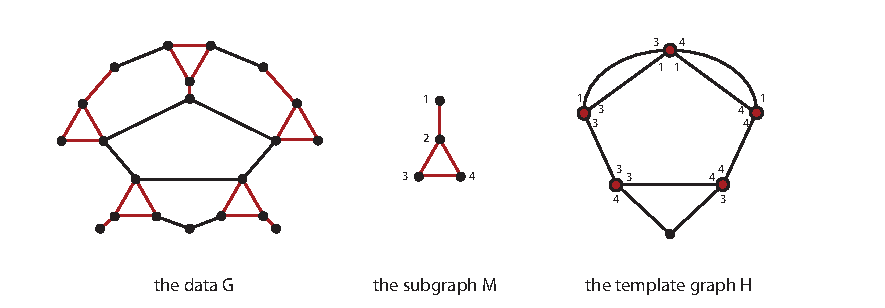
\includegraphics[width=\textwidth]{./images/illustration.pdf}
  \caption{An illustration of the motif code. We store $M$ once, and remove its instances from $G$, replacing them with a single, special node. The links to special nodes are annotated with `rewiring' information, which tells us how to rewire the subgraph back into $H$. Storing only $H$ and $M$ is enough to reconstruct the data.}
   \label{figure:motif-code}
\end{figure}  

\paragraph{Removing overlaps} The first thing we need is a subset $\cal I$ of ${\cal I}^\text{raw}$ such that the instances contained within it do not overlap: i.e. for each $I_a$ and $I_b$ in $\cal I$, we have $I_a \cap I_b = \emptyset$. To maximize the scalability of the algorithm, we will use a greedy approach to find a reasonable subset, rather than attempting to approximate an optimal solution.

As we will see later, the most important factor for compression is the number of links an instance has to nodes outside the instance. We call this the \emph{exdegree}.\footnote{Unlike the in- and outdegree, the exdegree is not a property of a node, but of a subgraph.} In order to find a subset of instances with low exdegree, we first sort ${\cal I}^\text{raw}$ by exdegree in ascending order. We then remove the first $I$, add it to our subset $\cal I$ and remove all other instances that overlap with it. We continue removing the first remaining instance until $\cal I$ is empty.

\paragraph{Encoding integers} In the following, we will often need to encode single natural numbers, or a sequence of natural number from a finite range. For single numbers, we will use the code corresponding to the probability distribution $p^\N(n) = 1/ (n(n+1))$, and denote it $L^\N(n)$.\footnotemark

\footnotetext{Note that this code is only used for storing single integers like graph dimensions, or the parameters of other codes. For long sequences of integers we use the DM code. Therefore, the specific choice of $p^\N(n)$ does not affect the codelength very much.}

For sequences of elements from a finite set, we use the code corresponding to a \emph{Dirichlet-Multinomial} (DM) distribution. Let $S$ be a sequence of length $k$ of elements from some alphabet $\Sigma$. Conceptually, the DM distribution models the following sampling process: we sample a probability vector $p$ on $[0, |\Sigma|]$ from a Dirichlet distribution with parameter vector $\alpha$, and then sample $k$ symbols from the categorical distribution represented by $p$. The probability mass function corresponding to this process can be expressed as
\begin{align*}
&p^\text{DirM}_\alpha(S\mid k, \Sigma) = \prod_{i \in [1,k]} \text{DirM}_\alpha(S_i\mid S_{1:i-1}, k, \Sigma) \\
&\text{DirM}_\alpha(S_i \mid S', k, \Sigma) = \frac{f(S_i, S') + \alpha_i}{|S'| + \sum_i \alpha_i}
\end{align*}
where $f(x, X)$ denotes the frequency of $x$ in $X$. We use $\alpha_i = 1/2$ for all $i$. Let $L^\text{DirM}_{k,\Sigma} (S) = -\log p^\text{DirM}(S \mid k, \Sigma)$. The DM model can be seen as encoding each element from $S_i$, using the smoothed relative frequency of $S_i$ in the subsequence $S_{1:i=1}$ preceding it. Thus the probability of a given symbol changes at each point in the sequence, based on how often it has been observed up to that point.

Note that this code is parametrized with $k$ and $\Sigma$. If these cannot be deduced from information already stored, they need to be encoded separately. When encoding natural numbers, we will have $\Sigma = [0, n_\text{max}]$, and we only need to encode $n_\text{max}$. A useful property of the DM code is that it is \emph{exchangeable}: if we re-arrange the elements of $S$, the codelength remains the same. 

Note that, since we use $L^\N(n)$ and $L^\text{DirM}(n)$ only in the motif code, there is no need for them to be optimal. The better they compress, the more motifs we will find, but we do not require optimal results for the algorithm to be valid. 

\paragraph{The motif code} We can now define the full motif code. It stores the following elements. Since each corresponds to a prefix-free code, we can simply concatenate their codewords for a prefix-free codeword for the data.
\begin{description}
\item[subgraph] First, we store the subgraph $M$ using $L^\text{base}(M)$ bits.
\item[template] We then create the \emph{template graph} $H$ by removing the nodes of each instance $I \in \cal I$, except for the first, which becomes a specially marked node, called an \emph{instance node}. The internal links of $I$---those incident to two nodes both in $I$---are removed from the graph. Any link connecting a node outside of $I$ to a node inside of $I$ is kept, and rewired to the instance node.
\item[instance nodes] $L^\text{base}$ does not record which nodes of $H$ are instance nodes, so we must record this separately. Once we have recorded how many instance nodes there are, there are $n(H) \choose |{\cal I}|$ possible placements, so we can encode this information in $L^\N (|{\cal I}|) + \log {n(H) \choose |{\cal I}|}$ bits. 
\item[rewiring] For each side of a link in $H$ incident to an instance node, we need to know which node in the motif it originally connected to. Let there be some agreed-upon order in which to enumerate the links of any given graph. Given this order, we only need to encode the sequence $W$ of integers $w_i \in [1,\ldots, n(M)]$. We do so using the DM model described above. The maximum symbol and length of $W$ can be deduced from parts already encoded. Note that this code is invariant to the ordering of $W$, so the particulars of the canonical node ordering do not need to be specified.
\item[multiple edges] Since $L^\text{base}$ can only encode simple graphs, we cannot use it to store $H$ directly, since collapsing the instances into single nodes may have created multiple edges. We remove all multiple edges and encode them separately. We assume a canonical ordering over the links and record for each link incident to an instance node, how many copies of it were removed. This gives us a sequence $R$ of natural numbers $R_i \in [0, r_\text{max}]$ which we store by first recording the maximum value in $L^\N(\max(R))$ bits, and then recording $R$ with the DM model.
\item[insertions] Finally, while $H$ and $M$ give us enough information to recover a graph isomorphic to $G$, we cannot yet reconstruct where each node of a motif instance belongs in the node ordering of $G$. Note that the first node in the instance became the instance node, so we only need to record where to insert the rest of the nodes of the motif. This means that we perform $|{\cal I}| (n(M)-1)$ such insertions. Each insertion requires $\log (t+1)$ bits to describe, where $t$ is the size of the graph before the insertion. We require $\sum_{t=n(H)}^{n(G)-1} \log (t+1) = \log (n(G)!) - \log (n(H)!)$ bits to record the correct insertions.
\end{description} 

\begin{pseudo}[th]
\caption{The motif code $L^\text{motif}(G ; M, {\cal I}, L^\text{base})$. Note that the nodes of the graph are integers.}
\label{algorithm:motif-code}
{ 
Given:\\ 
\tab a graph $G$, a subgraph $M$,\\ 
\tab a list $\cal I$ of instances of $M$ in $G$, a code $L^\text{base}$ on the simple graphs.\\
\\
$b_\text{subgraph} \leftarrow L^\text{base}(M)$\hfill \textbf{subgraph} \\
\\
\emph{\# replace each instance with a single node} \\
$H \leftarrow \text{copy}(G)$, $W = [] $\hfill \textbf{template} \\
\textbf{for each } $I = \{ m_1, \ldots m_{n(M)}\}$ \textbf{in} $\cal I$:\\
\tab \emph{\# We use $m_1$ (the $m_1$-th node in $G$) as the instance node}\\
\tab \textbf{for each} link $l$ between a node $n_\text{out}$ not in $I$ and a node $m_j$ in $I$:\\
\tab \tab \textbf{if} $j \neq 1$: add a link between $n_\text{out}$ and $m_j$\\
\tab \tab $W$.append$(j)$\\
\tab remove all nodes $m_i$ except $m_1$, and all incident links\\
$b_\text{rewiring} \leftarrow  L^\text{DirM}_{|W|, n(M)}(W)\hfill\textbf{rewiring}$\\
\\
\emph{\#Remove multiple edges from $H$  and record the duplicates in $R$}\\
$R, H' \leftarrow \text{simple}(H)$ \\
$b_\text{template} \leftarrow L^\text{base}(H')$\\ 
$b_\text{multi-edges} \leftarrow L^\N(\max(R)) + L^\text{DirM}_{|R|, \max(R)}(R)$ \hfill \textbf{multiple edges}\\
\\
$b_\text{instances} \leftarrow L^\N (|{\cal I}|) \log {n(H) \choose |{\cal I}|}$ \hfill \textbf{instance nodes}\\
$b_\text{insertions} \leftarrow \log (n(G))! - \log (n(H))!$ \hfill \textbf{insertions}\\    
\\
\textbf{return} $b_\text{subgraph} + b_\text{template} + b_\text{rewiring} + b_\text{multi-edges} + b_\text{instances} + b_\text{insertions}$\\
}
\end{pseudo} 

\paragraph{Pruning the list of instances} Since our code accepts any list of motif instances, we are free to take the list $\cal I$ and remove instances before passing it to the motif code, effectively discounting instances of the motif. This can often improve compression, as storing the rewiring information for instances with high exdegrees may cost more than we gain from removing them from the graph. We sort  $\cal I$ by exdegree and search for the value $c$ for which compressing the graph with only the first $c$ elements of $\cal I$ gives the lowest codelength.

The codelength $L^\text{motif}$ as a function of $c$ is roughly unimodal, which means that a ternary search should give us a good value of $c$ while reducing the number of times we have to compute the full codelength. We use a \emph{Fibonacci search} \citep{kiefer1953sequential}, an elegant variation on ternary search requiring only one sample per recursion.

\paragraph{Implementation} The \textbf{template} part of the code can be time and memory intensive to compute for large graphs, as it involves creating a copy of the data. For any given $L^\text{base}$, we can create a specific implementation which computes the codelength required for storing the template graph without constructing $H$ explicitly. This will speed up the computation of the code at the expense of creating a new implementation for each new null model. We use such specific implementations for our three null models.

More precisely, since we would like to operate efficiently on very large graphs, with a relatively low number of motif instances, we would like to avoid, where possible, operations requiring a full pass over the entire graph. We do this by storing the parameters of the null model (either the degree sequence or the size and number of links) for the complete graph, and computing how they change when the template graph is created. We can do this with a loop over the motif instances, computing directly how the model parameters change. Since the parameters determine the codelength, this is all we need to determine the number of bits required to store the template graph. In this computation we must make sure also to compute which links of the template graph become multiple links, and how many external links connect to each node within the motif. 

\section{Null Models}

\label{section:null-models}
We will define three null models. For each model we follow the same pattern: we first describe a parametrized model (which does not represent a code on all graphs). We then use this to derive a bound as described in Section~\ref{section:multiplerejection}, so that we can reject a set of null models, and finally we describe how to turn the parametrized model into a complete model to store graphs within the motif code.  

Specifically, let $L^\text{name}_\theta(G)$ be a parametrized model with parameter $\theta$. Let $\hat\theta(G)$ be the value of $\theta$ that minimizes $L^\text{name}_\theta(G)$ (the maximum likelihood parameter). From this we derive a bound $B^\text{name}(G)$---usually using $B^\text{name}(G) = L^\text{name}_{\hat\theta(G)}(G)$---which we will use in place of the null model. Finally, we create the complete model by two-part coding: $L^\text{name}(G) = L^{\theta}(\hat\theta(G)) + L^\text{name}_{\hat\theta(G)}(G)$. 

\subsection{The Erd\H{o}s-Renyi Model}
\label{section:null models}

The Erd\H{o}s-Renyi (ER) model is probably the best known probability distribution on graphs \citep{renyi1959random,gilbert1959random}. It takes a number of nodes $n$ and a number of links $m$ as parameters, and assigns equal probability to all graphs with these attributes, and zero probability to all others. This gives us 
\[
L^\text{ER}_{n, m}(G) = \log{(n^2-n)/2 \choose m} 
\] 
for undirected graphs, and 
\[
L^\text{ER}_{n, m}(G) = \log{n^2-n \choose m} 
\] 
for directed graphs. We use the bound $B^\text{ER}(G) = L^\text{ER}_{n(G), m(G)}(G)$.

For a complete code on simple graphs, we encode $n$ with $L^\N$. For $m$ we know that the value is at most $m_\text{max}=(n^2-n)/2$ in the undirected case, and at most $m_\text{max}=n^2-n$ in the directed case, and we can encode such a value in $\log (m_\text{max} + 1)$ bits ($+1$ because $0$ is also a possiblity). This gives us:
\[
L^\text{ER}(G) = L^\N(n(G)) + \log (m_\text{max} + 1) + L^\text{ER}_{\theta}(G)\;\text{with}\;\theta=(n(G),m(G))\p
\]
 
\subsection{The Degree-Sequence Model}
\label{section:degree-sequence-model}

The most common null model in motif analysis is the \emph{degree-sequence model}, also known as the \emph{configuration model} \citep{newman2010networks}. 
For undirected graphs, we define the degree sequence of graph $G$ as the sequence $D(G)$ of length $n(G)$ such that $D_i$ is the number of links incident to node $i$ in $G$. For directed graphs, the degree sequence is a pair of such sequences $D(G) = (D^\text{in}, D^\text{out})$, such that $D^\text{in}_i$ is the number of incoming links of node $i$, and $D^\text{out}_i$ is the number of outgoing links.

\paragraph{The parametrized model $L^\textnormal{DS}_D(G)$} The degree-sequence model $L^\text{DS}_D(G)$ takes a degree sequence $D$ as a parameter and assigns equal probability to all graphs with that degree sequence. Assuming that $G$ matches the degree sequence, we have $L^\text{DS}_D(G) = \log |\cG_D|$ where $\cG_D$ is the set of simple graphs with degree sequence $D$. There is no known efficient way to compute this value for either directed or undirected graphs, but various estimation procedures exist. We use an importance sampling algorithm discovered independently by \cite{blitzstein2011sequential} and \cite{charo2010efficient}.\footnotemark~This algorithm is guaranteed to produce any graph matching $D$ with some nonzero probability. Crucially, the algorithm does not backtrack or reject candidates, which means that if we multiply the probability of each random choice made in sampling, we get the probability of the sample under our sampling procedure. That is, the algorithm produces, along with a sample $G \in \cG_D$, the probability $q^\text{DS}_D(G)$ of the algorithm producing $G$. While the samples are not uniform, we do have
\begin{equation}
{E} \left [\frac{1}{q^\text{DS}_D(G)}\right] = |\cG_D| \label{line:expectation}
\end{equation}
where $G$ is a random variable representing a sample from the algorithm. Thus, we can sample a number of graphs and take the mean of their inverse probability under $q^\text{DS}_D$ to estimate $p^\text{DS}_D(G)$. This is a form of \emph{importance sampling}. 

\footnotetext{Specifically, our implementation uses the algorithms described in \cite{charo2010efficient} and \cite{kim2012constructing}. However the non-uniform sampling from the candidate set, discussed in \cite[p10, step 5]{blitzstein2011sequential} is crucial to achieving a low variance in the sampling distribution, and thus a fast convergence.}

Unfortunately, even with the highly optimized implementations described in \cite{charo2010efficient} and \cite{kim2012constructing} sampling can be slow for large graphs. Luckily, we are only interested in an estimate of the codelength accurate to around the level of single bits, which means that we only need to sample until we have a rough estimate of the order of magnitude of $|\cG_D|$. For instance, if we accept a margin of error of only 15 bits (of the potentially $10^6$ bits required to store the graph), we can underestimate the number of graphs by 4 orders of magnitude and still end up within the margin. All we need is a reliable confidence interval for our estimate, so that we can choose a suitably conservative bound. Our method of obtaining such a confidence interval is described in the appendix. In all cases, we use a one-sided confidence interval: when computing the codelength under the null model, we use a lower bound for the true value, and when computing the codelength for the motif code, we use an upper bound. Thus, the difference in codelength is a lower bound for the true value.

\paragraph{The bound $B^\textnormal{DS}(G)$} To get a bound for all two-part codes on $L^\text{DS}_D$, we could use ${B'}^\text{DS}(G) = L^\text{DS}_{D(G)}(G)$. Beating such a bound would tell us that no property of the degree sequence could explain the motif we had found. Unfortunately, the degree sequence forms a large part of the code, and a lot of evidence is required to compress better than ${B'}^\text{DS}(G)$ with a complete code. 

Instead, we make the assumption that the degrees are sampled independently from a single distribution $p^\text{deg}(n)$ on the the natural numbers. This corresponds to a code $\sum_{D_i \in D}L^\text{deg}(D_i)$ on the entire degree sequence. Let $f(s, D)$ be the frequency of symbol $s$ in sequence $D$. It can be shown that $B^\text{deg}(D) = \sum_{D_i \in D} f(D_i, D)/|D|$ is a lower bound for any such code on the degree sequence. This gives us the bound $B^\text{DS}(G) = B^\text{deg}(D(G))) + L^\text{DS}_{D(G)}(G)$. For directed graphs, we use $B^\text{DS}(G) = B^\text{deg}(D^\text{in}(G))) + B^\text{deg}(D^\text{out}(G))) + L^\text{DS}_{D(G)}(G)$.

Note that the \emph{scale-free} property of many complex graphs is captured by this model. Compressing better than $B^\textnormal{DS}(G)$ with a certain motif $M$, indicates that the occurrences of $M$ are not explained by the scale-freeness of the graph.

\paragraph{The complete model $L^\textnormal{DS}(G)$} For the alternative model we need a complete code. First, we store $n(G)$ with $L^\N$. We then store the maximum degree and encode the degree sequence with the DM model. For undirected graphs we get: 
\[
L^\text{DS}(G) = L^\N(n(G)) + L^\N(d) + L^\text{DirM}_{\theta}(D) + L^\text{DS}_{D(G)}(G) \;\text{with}\; \theta = \left(n(G), max(D)\right)
\]
and for directed graphs
\begin{align*}
L^\text{DS}(G) = &L^\N(n(G)) \\ 
 + &L^\N(\max(D^\text{in})) + L^\text{DirM}_{\theta}(D^\text{in})\\
 + &L^\N(\max(D^\text{out})) + L^\text{DirM}_{\phi}(D^\text{out}) + L^\text{DS}_{D(G)}(G) \\
 \text{with}&\; \theta = \left(n(G), \max(D^\text{in})\right), \phi = \left(n(G), \max(D^\text{out})\right) 
\end{align*} 

Note that in the computation of $L^\text{motif}$ with $L^\text{DS}$ as a base model, we estimate $|\cG_D|$ for both the template graph and the motif. It is important to combine the confidence intervals over these two estimates carefully, so that we end up with a correct confidence interval over the total codelength. This is discussed in the supporting materials. For $L^\text{motif}$, we compute a one-sided confidence interval to get an \emph{upper}bound, so that with 95\% confidence we are \emph{over}estimating the size of the motif code. 

\subsection{The Edgelist Model}

While estimating $|\cG_D|$ can be costly, we can compute an upper bound efficiently. Assume that we have a directed graph $G$ with $n$ nodes, $m$ links and a pair of degree sequences $D = (D^\text{in}, D^\text{out})$. To describe $G$, we might write down the links as a pair of sequences $(F, T)$ of nodes: with  $F_i$ the node from which link $i$ originates, and $T_i$ the node to which it points. Let $\cS_d$ be the set of all pairs of such sequences satisfying $D$. We have $ v$ possibilities for the first sequence, and $m \choose D_1^\text{out}, \ldots, D_n^\text{out}$ for the second. This gives us $|\cS_D| = {m \choose D_1^\text{in}, \ldots, D_n^\text{in}}{m \choose D_1^\text{out}, \ldots, D_n^\text{out}} = m!m! / \prod_{i=1}^n D^\text{in}_i ! D^\text{out}_i !$. We have $|\cS_D| > |\cG_D|$ for two reasons. First, many of the graphs represented by such a sequence pair contain multiple links and self-loops, which means they are not in $\cG_D$. Second, the link order is arbitrary: we can interchange any two different links, and we would get a different pair of sequences, representing the same graph, so that for a graph with no multiple edges, there are $m!$ different sequence-pairs to represent them. 

To refine this upper bound, let $\cS'_D \subset \cS_D$ be the set of sequence pairs representing simple graphs. Since all links in such graphs are distinct, we have $|\cG_D| = |\cS'_D|/m!$. Since $|\cS'_D| \leq |\cS_D|$, we have \footnotemark
\[
|\cG_D| \leq \frac{m!}{\prod_{i=1}^n D^\text{in}_i ! D^\text{out}_i !} \p
\]

\footnotetext{This value was previously used in \cite{bezakova2006graph} as a precise value for the number of graphs with multiple edges. This is incorrect, as we can only divide by $m!$ if we know that no graphs have multiple edges.}

In the undirected case, we can imagine a single, long list of nodes of length $2m$. We construct a graph from this by connecting the node at index $i$ in this list to the node at index $m+i$ for all $i \in [1, m]$. In this list, node $a$ should occur $D_a$ times. We define $\cS_D$ as the set of all lists such that the resulting graph satisfies $D$. There are $(2m)! \choose D_1, \ldots, D_n$ such lists.
We now have an additional reason why $|\cS_D| > |\cG_D|$: each pair of nodes describing a link can be swapped around to give us the exact same graph. This gives us:
\[
|\cG_D| \leq |\cS'_D| / (2^m m!) = \frac{(2m)!}{2^m m! \prod_{i=1}^n D_i!} \p
\]

In both cases, the fact that we have an upperbound gives us a code: while the code as described assigns some probability mass to non-simple graphs, we can easily assume that this is assigned instead to some null-element, since we are only interested in the codelengths and probabilites of simple graphs. This gives us the following parametrized code for directed graphs:
\[
L^\text{EL}_D(G) = \log m! - \sum_{i=0}^n \log D_i^\text{in}! - \sum_{i=0}^n \log D_i^\text{out}!   
\]
where $(D^\text{in}, D^\text{out})$ are the degree sequences of $G$, and for the undirected case:
\[
L^\text{EL}_D(G) = \log (2m)! - \log m! - m - \sum_{i=0}^n \log D_i! \p   
\]

For the bound and the complete model, we follow the same strategy we used for the degree-sequence model: $B^\text{EL}(G) = B^\text{deg}(G) + L^\text{EL}_{D(G)}(G)$ and, 
\[
L^\text{EL}(G) = L^\N(n(G)) + L^\N(\max(D)) + L^\text{DirM}_{\theta}(D) + L^\text{EL}_{D(G)}(G) \;\text{with}\; \theta=(n(G), \max(D))
\] for undirected graphs and 
\begin{align*}
L^\text{EL}(G) = &L^\N(n(G)) \\ 
 + &L^\N(\max(D^\text{in})) + L^\text{DirM}_{\theta}(D^\text{in})\\
 + &L^\N(\max(D^\text{out})) + L^\text{DirM}_{\phi}(D^\text{out}) + L^\text{EL}_{D(G)}(G)\\
 \text{with}&\; \theta=(n(G), \max(D^\text{in})), \phi=(n(G), \max(D^\text{out})) \
\end{align*} for directed graphs.

\section{Experiments}

\label{section:experiments}

To validate and illustrate our method, we will perform four experiments. First, we will construct a graph by injecting instances of a single motif into a random network. The method should then recover only this motif as significant. Second, we will run the method on data sets from four different domains, and show the results for the most frequent subgraphs, using the three null models we have described. Third, we use the motifs identified by our method, and by the traditional approach, as features in a classification task, showing comparable performance, well above chance. This tells us that, at least for the purposes of classification, the motifs returned by our method are no less informative than those found by the traditional method. Finally, to show the scalability of the method with fast null models, we will run the analysis on several large graphs, first using purely memory based methods, and then with a disk-backed datastructure to store the graph.

In all experiments we search for motifs by sampling, based on the method described by \citet{kashtan2004efficient}. Note that we have no particular need for a sampling algorithm which provides an accurate approximation of the actual frequencies present in the graph, so long as it can provide us with a large selection of non-overlapping instances with low exdegree. For this reason, we adapt the algorithm to improve its speed: we start with a set $N'$ containing a single random node drawn uniformly. We then add to $N'$ a random neighbour of a random member of $N'$, and repeat until $N'$ has the required size. We extract and return $G[N']$. In the case of a directed graph, nodes reachable by incoming and outgoing links are both considered neighbours.  

The size $n(M)$ of the subgraph is chosen before each sample from a uniform distribution over the interval $[n_\text{min}, n_\text{max}]$. This distribution over sizes is biased towards small motifs: since there are fewer connected graphs for small sizes, small graphs are more likely to be sampled. As the results show, however, the method still finds motifs with many nodes, so we opt for this simple, ad-hoc method.

We re-order the nodes of the extracted graph to a canonical ordering for its isomorphism class, using the Nauty algorithm \citep{mckay1981practical}. We maintain a map from each  subgraph in canonical form to a list of instances found for the subgraph. After sampling is completed, we end up with a set of potential motifs and a list of instances for each, to pass to the motif code described in Section~\ref{section:motif-code}.

In all experiments, we report the \emph{log-factor}: $B^\text{null}(G) - L^\text{motif}(G; M, {\cal I}, L^\text{null})$. That is, we use the bound in place of the null model, and the complete code of the same null model is used in the motif code (to store the template graph and the motif). If the log-factor is larger than 10 bits, we can interpret it, as described in Section~\ref{section:model-selection}, as a successful hypothesis test, allowing us to reject the null model at $\alpha=0.001$. In all cases, a negative log-factor means that we do not have sufficient evidence to reject the null model, but a different experiment might yet achieve a positive log-factor. This could be achieved by sampling more subgraphs, using a different algorithm to find motif instances or taking more samples from the degree-sequence estimator.

All experiments in this paper were run on a single machine with a 2.60 Ghz Intel Xeon processor (E5-2650 v2) with 64 Gigabytes of memory and 8 physical cores. The memory and cores available to the program differ per experiment and are reported where relevant. 

\subsection{Recovering Motifs from Generated Data}

\label{section:recovering}

We use the following procedure to sample an undirected graph with $5000$ nodes and $10000$ links, containing $k$ injected instances of a particular motif $M$ with $n'$ nodes and $m'$ links. Let $M$ be given (in our experiment $M$ is always the graph indicated in red in Figure~\ref{figure:plot-synthetic}).

\begin{enumerate}
  \item Let $n = 5000 - (n'-1)k$ and $m = 10000 - m'k$ and sample a graph $H$ from the uniform distribution over all graphs with $n$ nodes and $m$ links.   
  \item Label $k$ random nodes, with degree 5 or less, as instance nodes.
  \item Let $p^\text{cat}$ be a categorical distribution on $\{1, \ldots, 5\}$, chosen randomly from the uniform distribution over all such distributions.
  \item Label every connection between an instance node and a link with a random value from $p^\text{cat}$. Links incident to two instance nodes, will thus get \emph{two} values.
  \item Reconstruct the graph $G$ from $M$ and $H$.
\end{enumerate}


\begin{figure*}[tb]
  \hspace{-0.1\textwidth}
  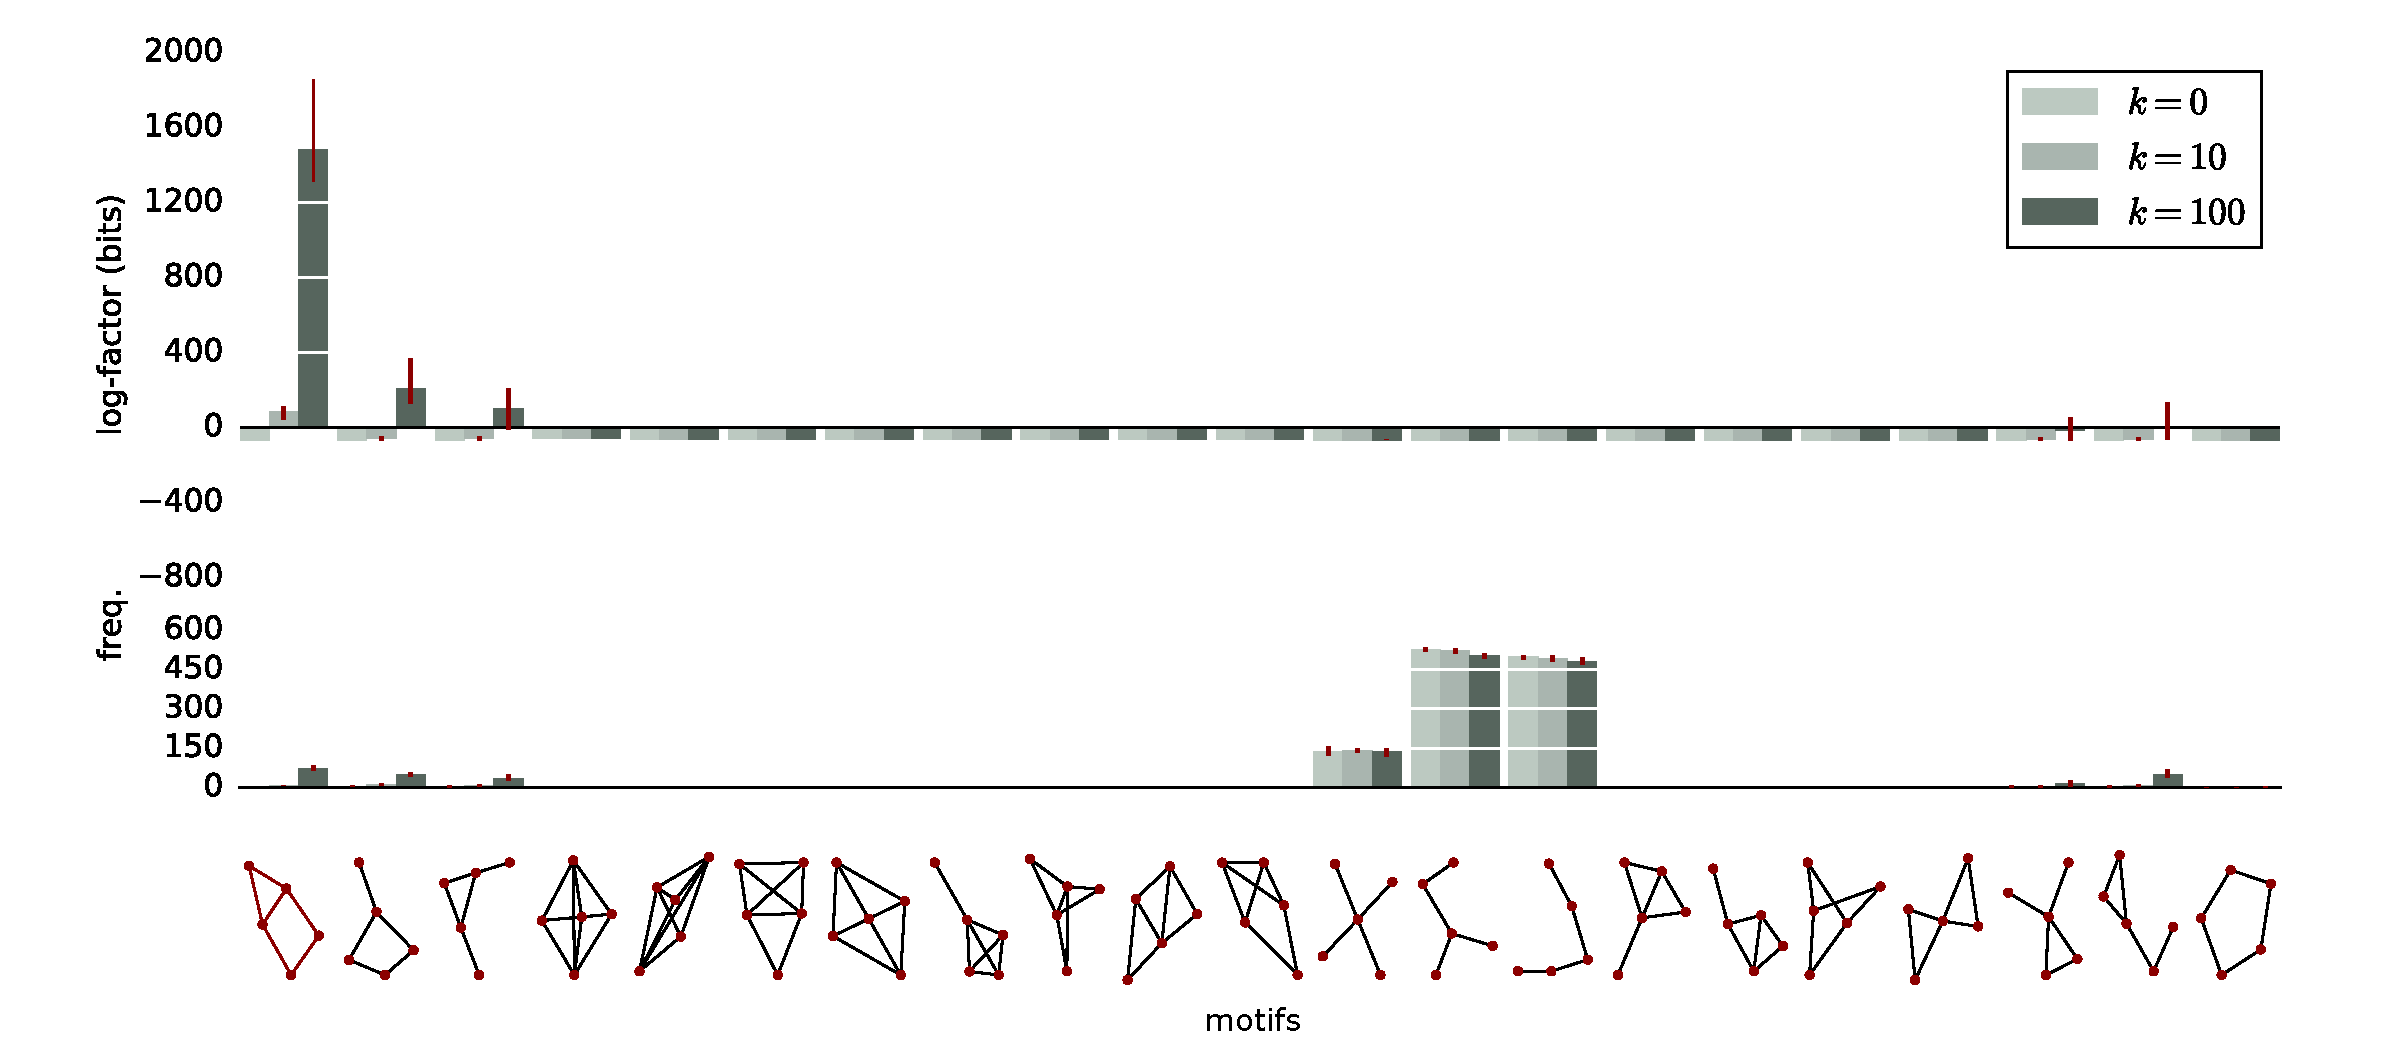
\includegraphics[width=1.2\textwidth]{./images/synthetic-plot.pdf}
  \caption{\small The results of the experiment on generated data. The bottom row shows all 21 simple connected graphs with 5 nodes (up to isomorphism). The middle row shows the number of non-overlapping instances found by the sampling algorithm for $k = 0$, $k=10$ and $k=100$ from left to right, for each motif. The bars show the average value over 10 randomly sampled graphs, with the same subgraph (shown in red) injected each time. The top row shows the difference between  the code length under the null model (the ER model) and under the motif code. Error bars represent the \emph{range}, i.e. they are drawn from the smallest to the largest observation.}
  \label{figure:plot-synthetic}
\end{figure*}

This is roughly similar to sampling from our motif code. In this graph, $M$ should be the only significant motif, with the exception of motifs that can be explained from the prevalence of $M$, ie. subgraphs and supergraphs of $M$, or graphs that contain part of $M$. However, these should have a markedly lower log-factor than $M$. For our experiment, we will only extract subgraphs of size 5, to rule out the first two cases.

On this sampled graph, we run our motif analysis. We run the experiment multiple times, with $k = 0$, $k = 10$ and $k = 100$, using the same subgraph $M$ over all runs, but sampling a different $H$ each time. For each value of $k$, we repeat the experiment 10 times. Per run we sample 5000 motifs. This value is chosen to show that even a very \emph{low} sample size is sufficient to recover the motif. The null model in all cases is the ER model, as that corresponds to the source of the data.

Figure~\ref{figure:plot-synthetic} shows the results for the 21 possible connected simple graphs of size 5. This result shows that, on such generated data, the method behaves as expected in the following ways:
\begin{itemize}
	\item If no motifs are injected---that is, the graph is sampled from the null model---no subgraphs are motifs.
	\item For a small number of injected motifs ($k = 10$), the correct motif is given a positive log-factor. Other subgraphs are shown to have very high frequencies, but the method correctly gives these a negative log factor. In other words, these are shown to be natural consequences of the null model.
	\item If the number of motifs is high ($k = 100$), the resulting significance increases. Note that in the traditional method, a such high significances require many more samples from the null model.
\end{itemize}

We can also see that once we insert 100 instances of the motif, two other subgraphs ``become motifs'': in both cases, these share a part of the inserted motif (a rectangle and a triangle). This is an important lesson for motif analysis: not every significant subgraph represents a meaningful result, some may be a byproduct of other motifs. This effect is not unique to our method, but occurs in all motif analysis.

\subsection{Motifs from Real-World Data}
\label{section:various}

Next, we show how our our approach operates on a selection of data sets across domains. Our main aim with this experiment is to show how the three null models influence the results. Specifically, to ascertain whether the edgelist model provides a reasonable approximation for the degree-sequence model.

We use the following data sets:
\begin{description}
\item[kingjames (undirected, $n=1773, m=9131$)] Co-occurrences of nouns in the text of the King James Bible \citep{konect:2014:moreno_names,konect:harrison}. Nodes represent nouns (places and names) and links represent whether these occur together in one or more verses. The full motif analysis took 23 hours and 16 minutes. 
\item[yeast (undirected, $n=1528, m=2844$)] A network of the protein interactions in yeast, based on a literature review \citep{reguly2006comprehensive}. Nodes are proteins, and links are reported interactions between proteins. We removed 81 self-loops. The full motif analysis took 3 hours and 19 minutes. 
\item[physicians (directed, $n=241, m=1098$)] Nodes are physicians in Illinois \citep{konect:2015:moreno_innovation,konect:coleman1957}. Links indicate that one physician turns to the other for advice. The full motif analysis took 31 minutes. 
\item[citations (directed, $n=1769, m=4222$)] The arXiv citation network in the category of theoretical astrophysics, as created for the 2003 KDD Cup \citep{gehrke2003overview}. To create a workable graph, we follow the procedure outlined in \citet{carstens2013motifs}: we include only papers published before 1994, remove citations to papers published after the citing paper, and select the largest connected component. The full motif analysis took 8 hours and 53 minutes. 
\end{description}
All data sets are simple (no multiple edges, no self-loops). In each case we take $5 \cdot 10^6$ samples with $n_\text{min} = 3$ and $n_\text{max} = 6$. We test the 100 motifs with the highest number of instances (after overlap removal), and report the log-factor for each null model. For the edgelist and ER models we use a Fibonacci search at full depth, for the degree-sequence model we restrict the search depth to $3$. For the degree-sequence estimator, we use $40$ samples and $\alpha=0.05$ to determine our confidence interval. We use the same set of instances for each null model.

\begin{figure*}[p]
  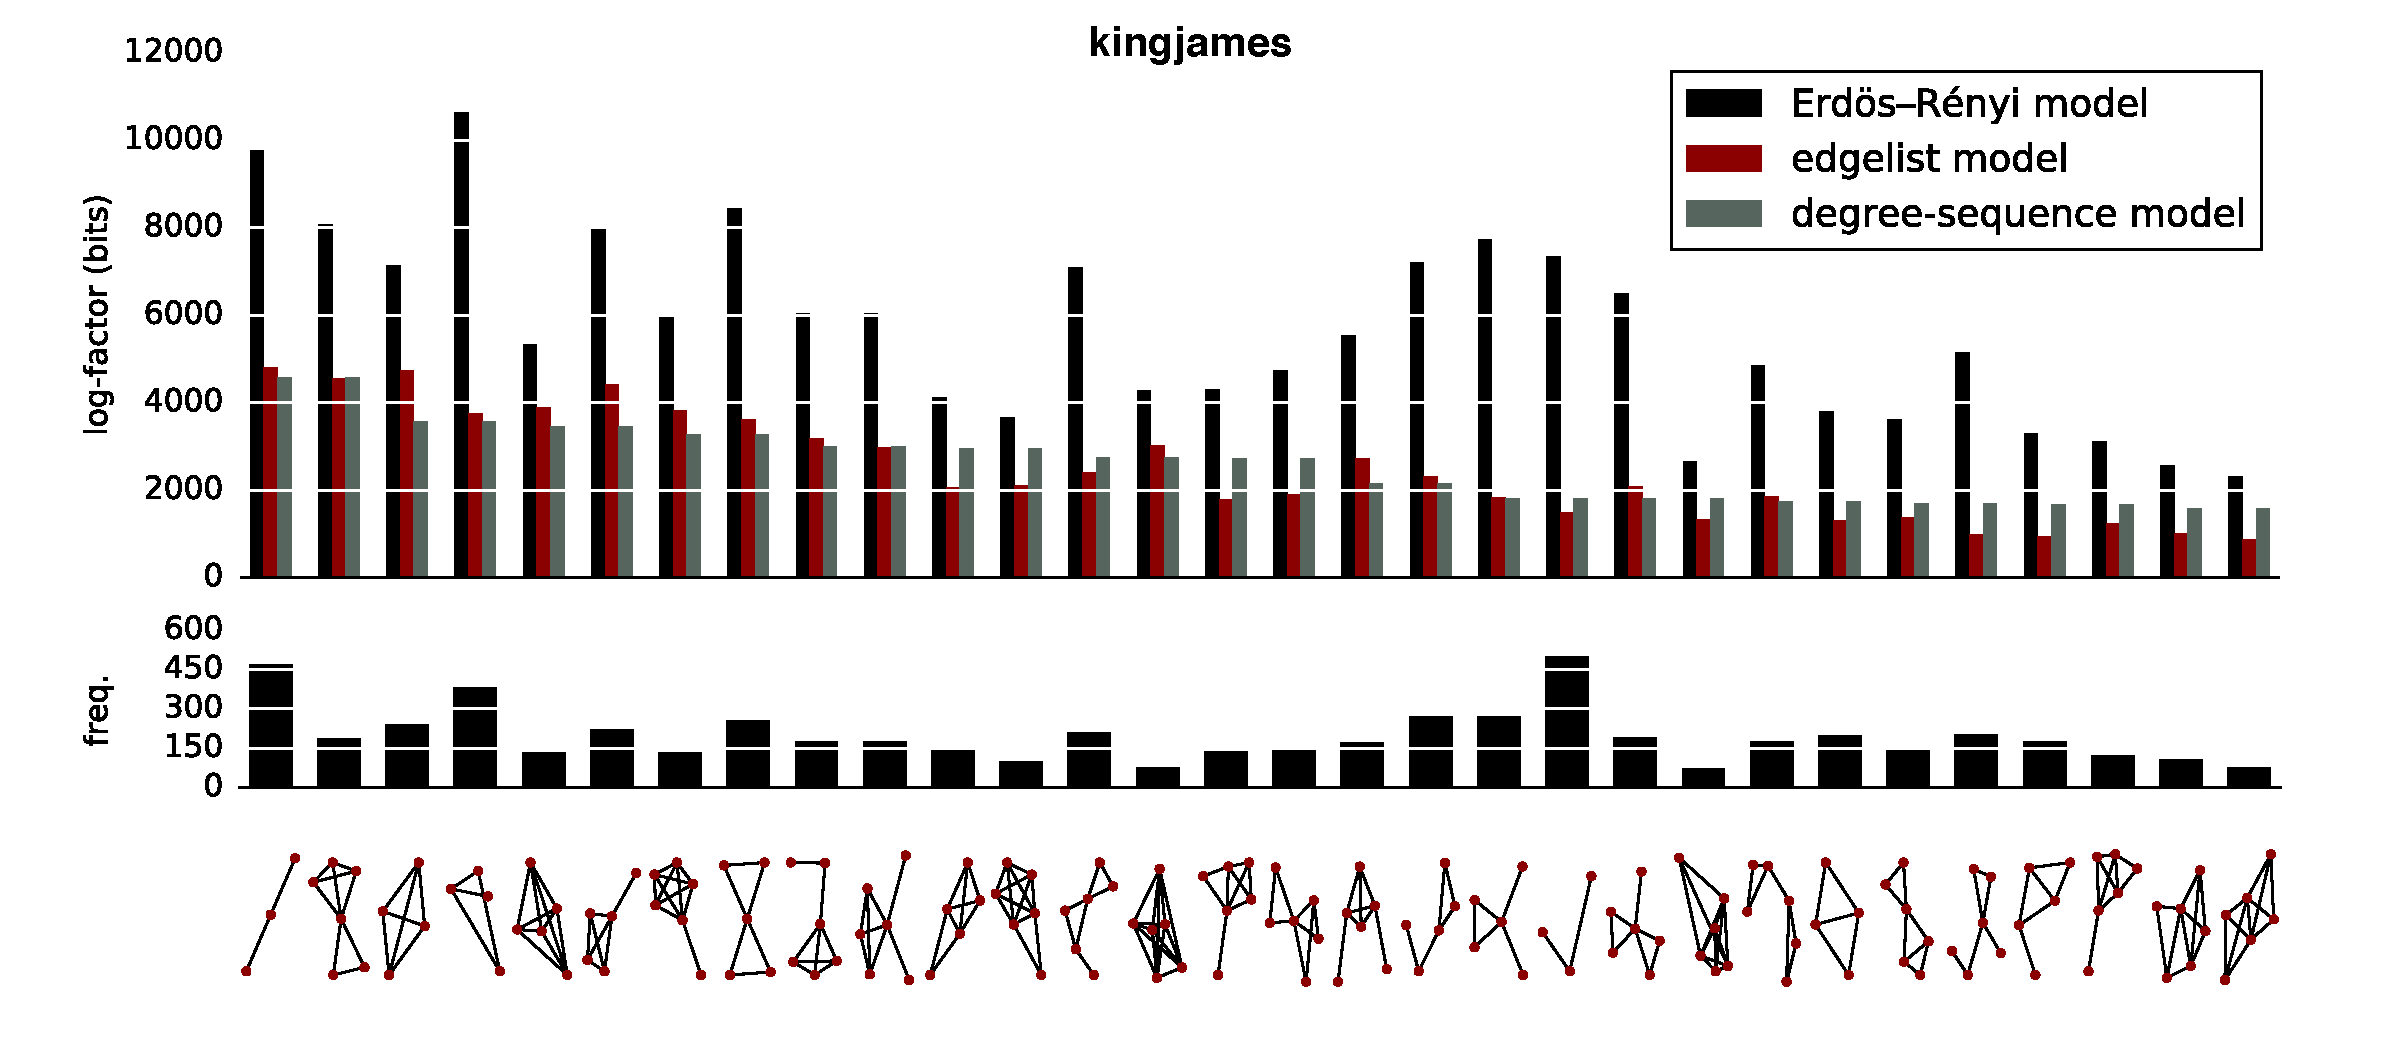
\includegraphics[width=\textwidth]{./images/kingjames/compare-plot.pdf}\\
  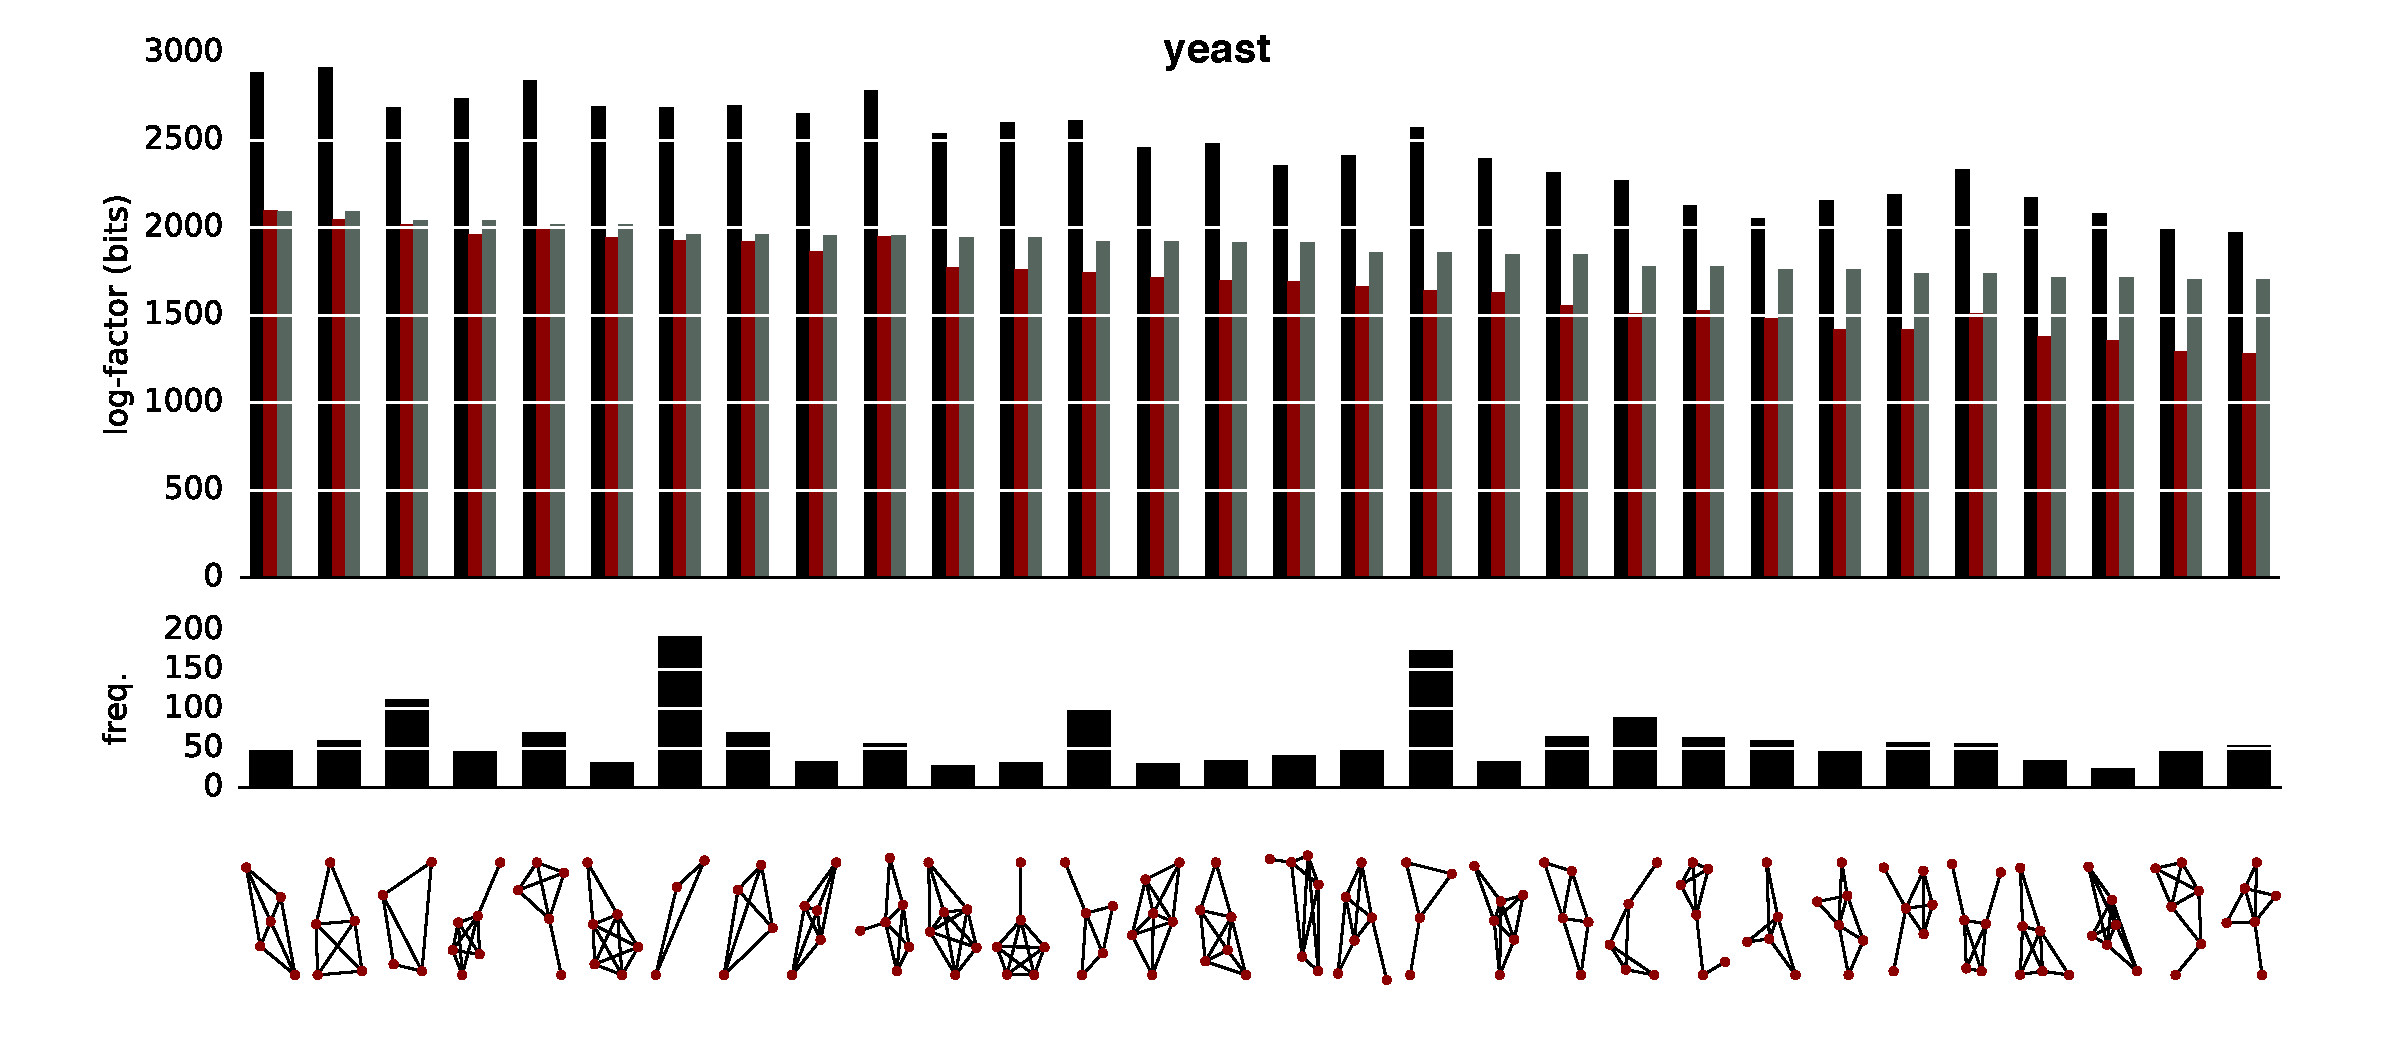
\includegraphics[width=\textwidth]{./images/yeast/compare-plot.pdf}\\
  \caption{The results of the motif extraction on the 2 undirected networks.}
  \label{figure:plot-und}
\end{figure*}
  
\begin{figure*}[p]
  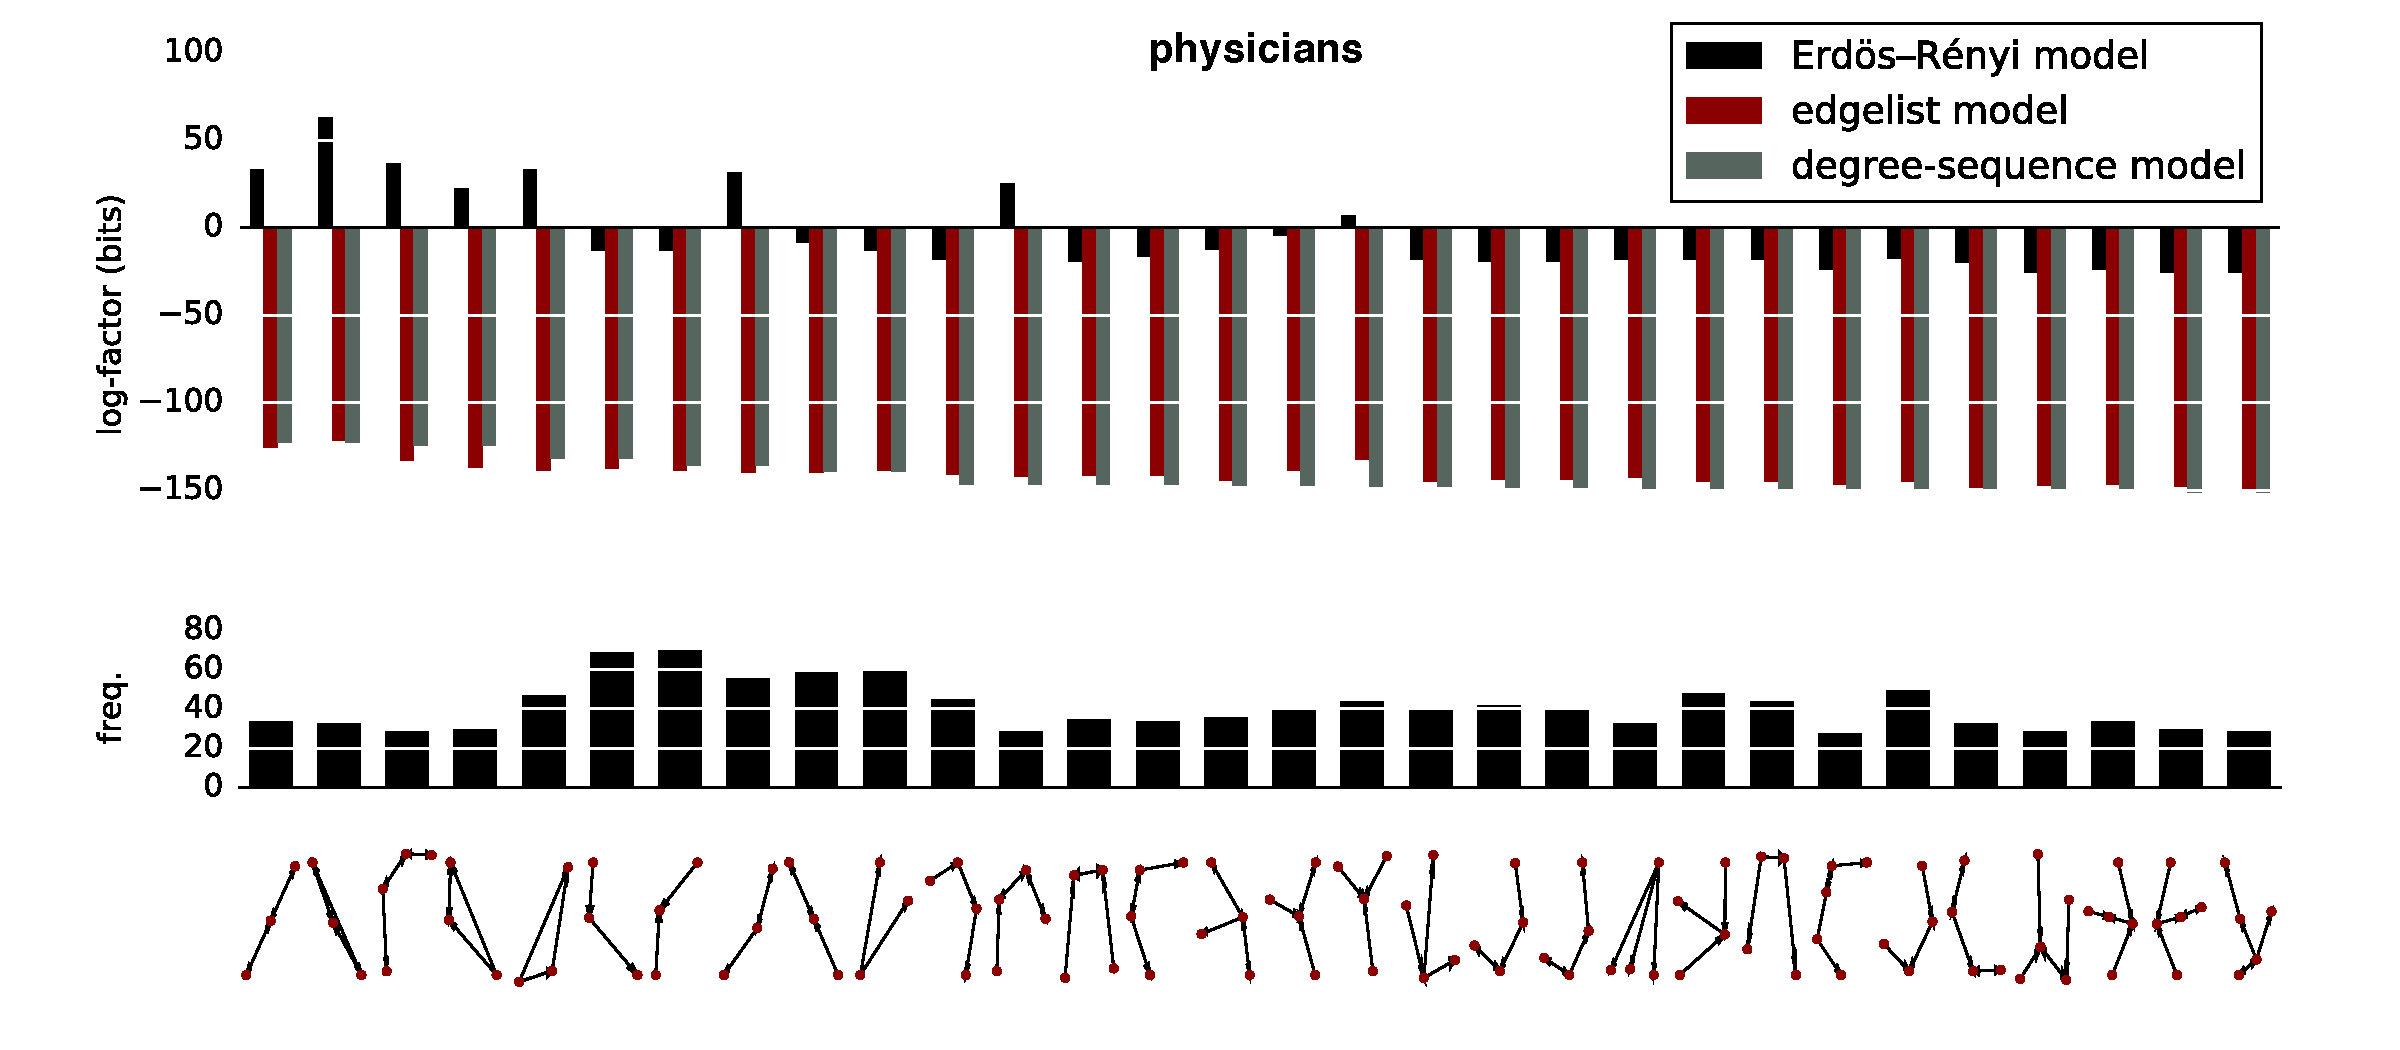
\includegraphics[width=\textwidth]{./images/physicians/compare-plot.pdf}\\
  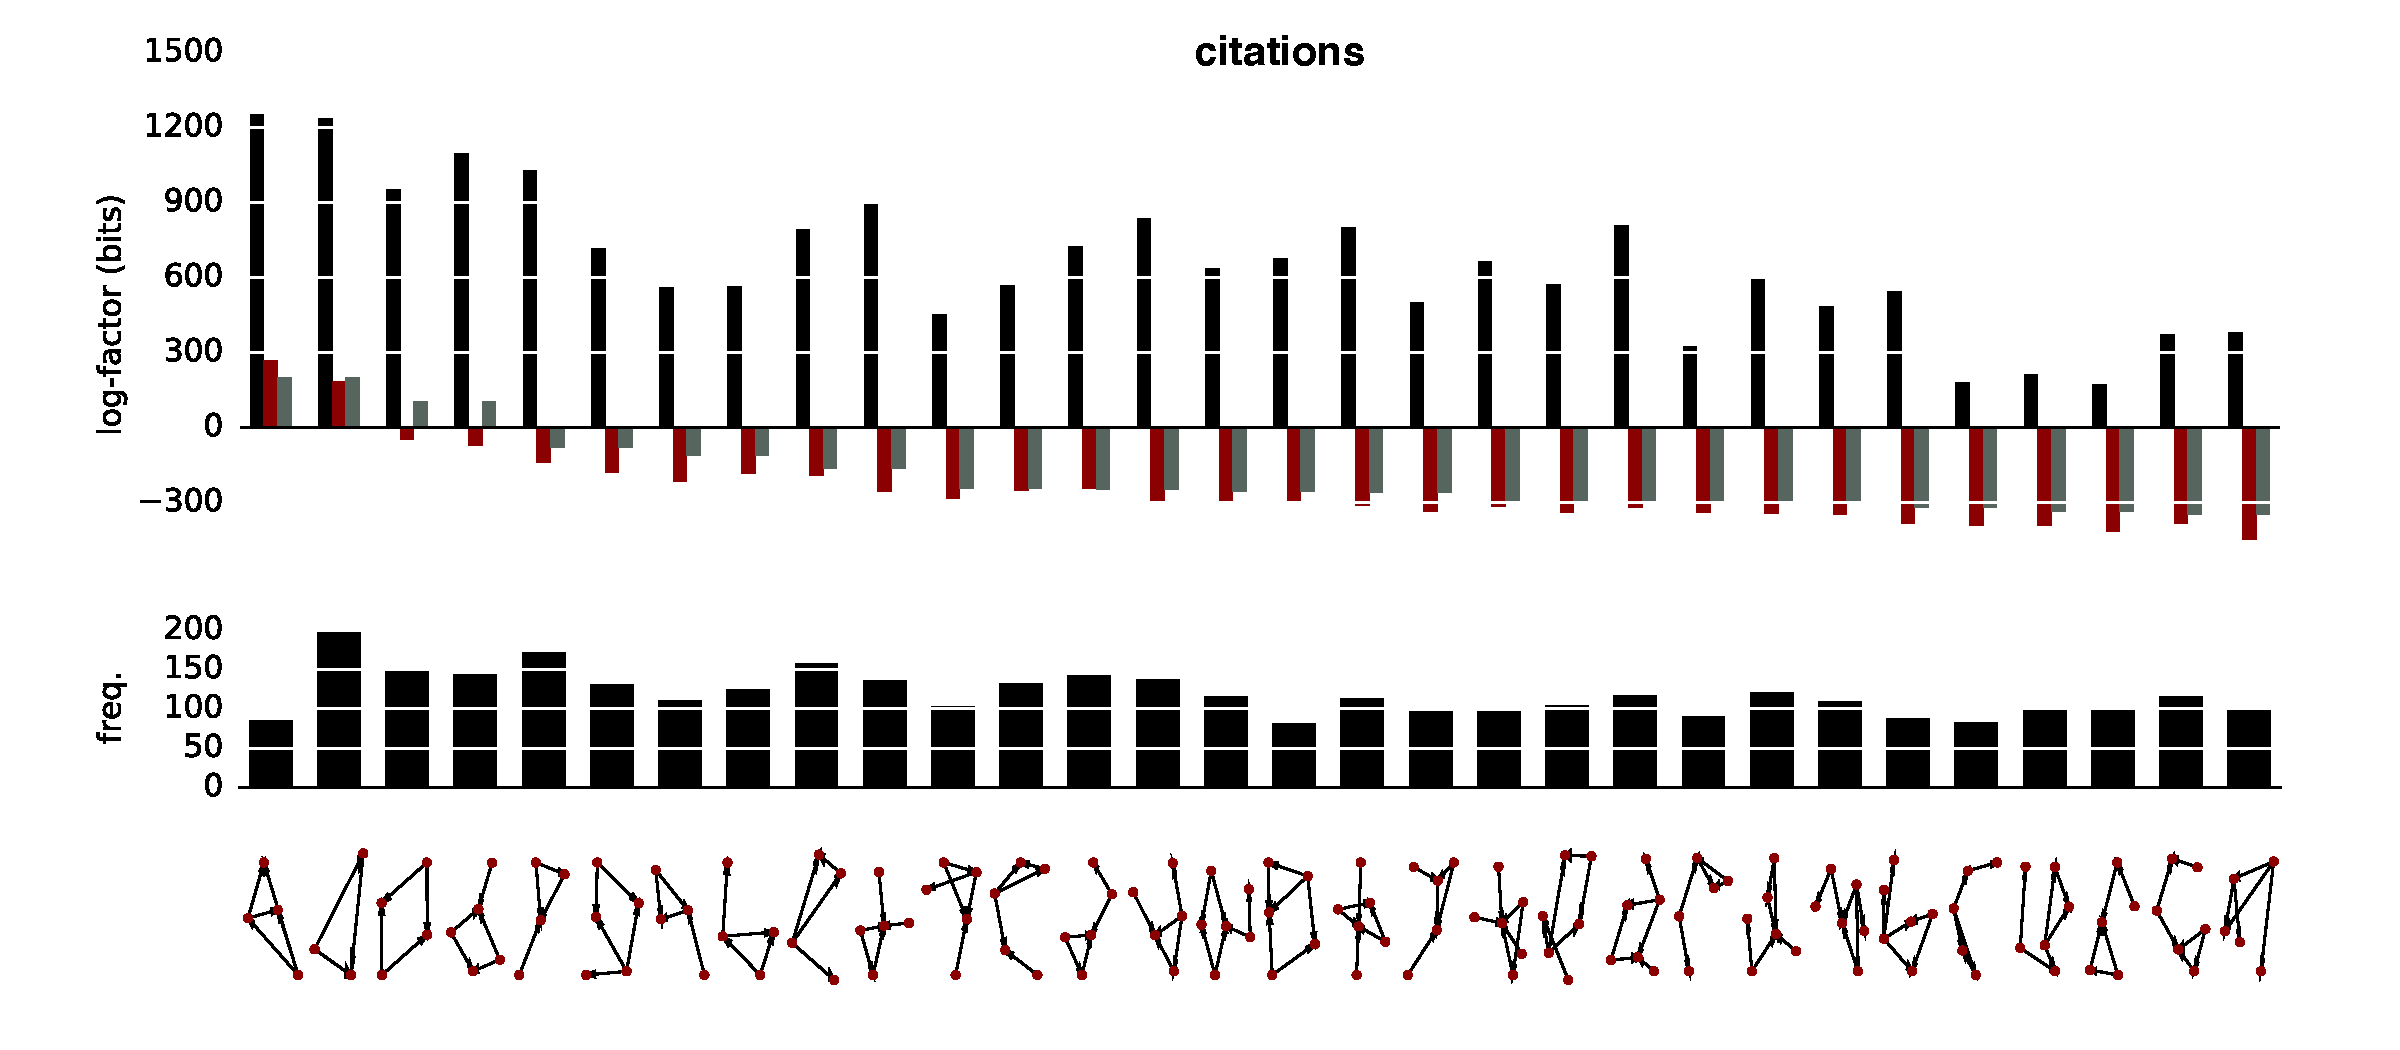
\includegraphics[width=\textwidth]{./images/citations/compare-plot.pdf}\\
  \caption{The results of the motif extraction on the 2 directed networks.}
  \label{figure:plot-dir}
\end{figure*}

The negative log-factors in some of the results may appear surprising at first, since the motif code should never do worse than the null model by more than a few bits: in the worst case, it can simply prune all motif instances, and use the null model for the entire graph. The negative values shown here are due to the use of a \emph{bound} for the parameters: the motif code must store the degree sequence explicitly, while the null model uses a lower bound for that part of the code.

Our first observation is that for the physician data set, there are no motifs under the degree-sequence null model. This likely because the physicians network is too small: the use of a bound for the null model means that the alternative model requires a certain amount of data before the differences become significant. Note, however, that if we were to compare against a complete model (instead of the bound), a constant term would be added to all compression lengths under the null model. In other words, the ordering of the motifs by relevance would remain the same.

In both the kingjames and the yeast graphs, many motifs contain cliques or near-cliques. This suggests that the data contains local communities of highly interconnected nodes which the null model cannot explain.

Finally, we would like to emphasize the scale of the null-hypothesis rejections. In the kingjames test, the most significant motif under the DS model has a log-factor of over 3500 bits. This corresponds to a rejection of the null model at significance $\alpha = 2^{-3500} \approx 10^{-1050}$. Note that accurate estimates of strong significances are a common problem in the traditional approach, since this requires very high numbers of samples from the null model \citep{picard2008assessing}.

For the experiments in this section, the maximum Java heap space was set to 2 Gigabytes. The computation of the log-factor of each motif was done in parallel, as was the sampling for the degree sequence model, with at most 16 threads runnning concurrently, taking advantage of the 8 available (physical) cores. 

Now, clearly, these analyses took relatively long, for data sets that are of medium size. The bottleneck here is the computation of the degree-sequence model. If we eliminate that, as we do in Section~\ref{section:large}, we see that we can run the same analysis in minutes on graphs that are many orders of magnitude larger than these. Moreover, the plots show a reasonable degree of agreement between the EL model and the DS model, suggesting that the former might make an acceptable proxy. But are the motifs returned still, in some sense, informative? We investigate this in the next section, comparing the traditional method of motif detection to our method, using the EL model. 

\subsection{Comparison with the traditional method}

\label{section:classification}

\begin{figure}[tbh]
{
  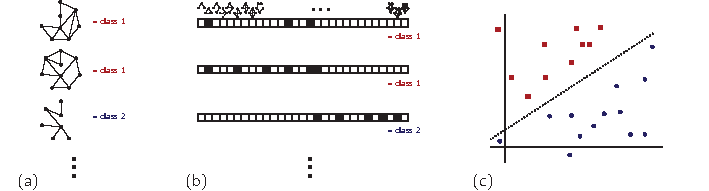
\includegraphics[width=\textwidth]{./images/experimentexplanation.pdf}	
}

  \caption{A schematic illustration of the classification experiment. (a) We start with a classification task on simple, undirected graphs. (b) These graphs are reduced to 29-dimensional binary feature vectors. Each feature corresponds to an undirected, connected mini-graph of size 3, 4, or 5. If the motif algorithm considers the mini-graph a motif for the current instance, the feature is 1, otherwise it is 0. This reduces the entire graph to just 29 bits of information, using only the judgements of the motif algorithm to represent the graph. If these judgements do indeed contain some information that characterises the graph, these feature vectors should be sufficient to perform better than a majority class classifier. (c) We apply a simple, linear SVM in the 29-dimensional feature space to perform the classification task on just the motif judgments.}
  \label{figure:experiment-explanation}
\end{figure}

Pattern mining on graph data is a very difficult task to evaluate. Not only is it unsupervised, we also have no ground truth data for what people might consider interesting subgraphs. Often, we do not even know what such a ground truth would look like: even a domain expert may not recognize a ``correct'' motif at first sight. Nevertheless, we have rather stretched the definition of a motif---choosing a different statistic, and an approximation to the default null model---so we need some assurance that after all this, the motifs found by our method are not completely meaningless.

The definition of what constitutes a good motif is exceedingly vague: papers variously describe a motif as a ``functional unit'', a ``characteristic pattern'' or a ``statistically significant subgraph.'' To be able to operationalize the definition into something that we can test empirically, we will define a network motif as a subgraph that is \emph{characteristic} for the full graph. That is, in some manner, the information that $M$ is a motif for $G$ should \emph{characterize} $G$: it distinguishes $G$ from the graphs for which $M$ is not a motif, and that distinction should be meaningful in the domain of the data.

Using this definition, we can test how effective a motif detection method is, using a graph classification task. We start with a set of undirected simple graphs, with associated classes. We then translate each graph into a binary feature vector using \emph{only the motif judgements} of the algorithm under evaluation. We test all connected subgraphs of size 3, 4, and 5, giving us 29 binary features. As we established in the previous paragraph, a good motif characterizes a graph in a way that is relevant to its domain. In the case of a graph classification task we are provided with a domain-relevant distinction in the form of the classes provided. If a simple classifier (in our case a linear SVM) can classify the graphs purely on the basis of these 29 motif judgments, the algorithm has succeeded in characterizing the graph. This approach---quantifying unsupervised pattern extraction through classification---was also used by \citet{leeuwen2006compression}. 

Our main aim is to establish that the resulting classifier performs better than chance. For this purpose we compare it to a majority class baseline. Our secondary aim is to show that we do not perform much worse than the traditional method. Note that our method allows motif analysis to scale up by at least four orders of magnitude, so we consider a small reduction in classification accuracy acceptable, so long as the method still significantly outperforms the majority class baseline.

Finding a graph classification task that fits our requirement is not easy: the graphs must be large enough to provide our method with enough data,\footnotemark~but small enough that the traditional method works without approximation. Moreover, the graphs must be undirected, so that we can use the highly efficient ORCA algorithm \citep{hovcevar2014combinatorial} to get exact subgraph counts for the traditional method. In order to tune the graph classification tasks to our needs, we adapt them from classification tasks on knowledge graphs, described in \cite{ristoski2016collection}. In these tasks, the data consists of a single labeled, directed multigraph, and the task is to predict classes for a specific subset of nodes (the \emph{instance nodes}). We translate the graph to an unlabeled simple graph by using the same nodes (ignoring their labels) and connecting them with a single undirected edge only if there are one or more directed edges between them in the original knowledge graph. 

\footnotetext{For smaller graphs our method can be adapted by testing against a single model, instead of using a bound to reject multiple null models as described in Section~\ref{section:model-selection}. However, for this test, we would like to evaluate the method as we expect it to be used.}

This gives us a classification task on the nodes of a single, undirected simple graph. We turn this into a classification task on \emph{separate} graphs by extracting the 3-neighborhood around each instance node. To control the size of the extracted neighborhoods, we remove the $h$ nodes with the highest degrees from the data before extracting the neighborhoods. $h$ was chosen by trial-and-error, before seeing the classification performance, to achieve neighborhoods with around 1000--2000 nodes.

We now have a graph classification task from which we can create feature vectors as described above. For our method, we sample 100 000 subgraphs, with size 3, 4, 5 having equal probability and test the compression levels under the edgelist model. We judge a subgraph to be a motif if it beats the EL bound by more than $- \log \alpha$ bits with $\alpha = 0.05$. 

Many methods for motif analysis have been published, but most are approximations or more efficient counting algorithms. Therefore, a single algorithm based on exact counts can act as a representation for most of the existing approaches. We perform exact subgraph counts on both the data and 1000 samples from the DS model. The samples from the null model are taken using the Curveball algorithm \citep{strona2014fast,carstens2016curveball}. We estimated the mixing time to be around 10 000 steps, and set the run-in accordingly. The subgraph counts were performed using the ORCA method.\footnote{We created a Java implementation, available at \url{https://github.com/pbloem/orca}.} We mark a subgraph as a motif if fewer than 5\% of the graphs generated from the DS model have more instances of the subgraph than the data does.\footnotemark~

\footnotetext{Note that the commonly used z-score method is seriously flawed, as discussed by \citet{picard2008assessing}, so we do not use it here.}

For performance reasons, we use only 100 randomly chosen instances from the classification task. On these 100 instances, we perform five-fold cross-validation.
We repeat the complete experiment, from sampling instances to cross-validation, 10 times. The classifier is a linear SVM ($C=1$). For tasks with more than 2 classes, the one-against-one approach \citep{knerr1990single} is used.

Note that the accuracy should not be compared to that achieved by others on these benchmarks, as we have thrown away almost all information in the original knowledge graph. We are merely using classification accuracy as a proxy for the quality of motif analysis. 

\begin{figure}[tbh]
{
  \begin{center}
  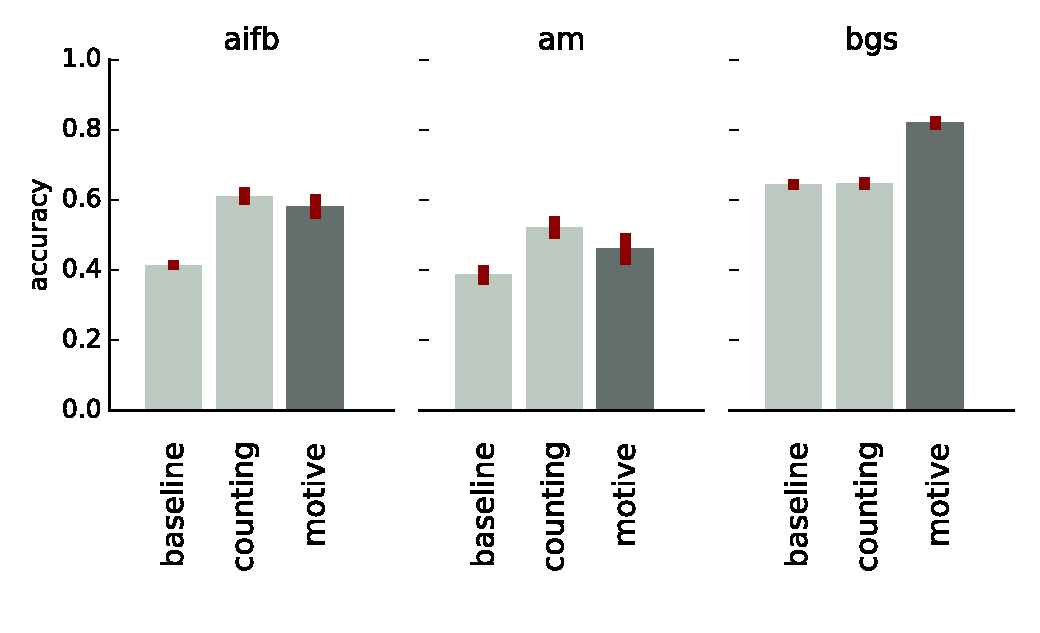
\includegraphics[width=0.8\textwidth]{./images/bars.pdf}
	\begin{tabular}{ r | r r r r r r}
		data & \# nodes & \# links & $h$ & $K$ & $\overline{n}$ & $\overline{m}$ \\
		\hline
		AIFB & 8 275 & 17 911 & 10 & 4 & 1877.11 & 7141.48 \\
		AM   & 1 495 566 & 2 393 604 & 3 000 & 11 & 2506.07 & 4392.06 \\
		BGS  & 333 613 & 362 627 & 250 & 2 & 3097.47 & 4404.49 \\
		\hline
	\end{tabular}
	\end{center}	
}

  \caption{The results of the classification experiment for the traditional method (`counting') and ours (`motive'). The bars show the mean accuracy of ten runs (with five-fold cross-validation performed within each run. The error bars show a 95\% confidence interval (assuming normality). The baseline shows the performance of a majority-vote classifier which ignores the features.  The table shows the size of the data, the average size and number of links ($\overline{n}$, $\overline{m}$) of the instance graphs, the number of classes $K$ and the number $h$ of hubs removed.}
  \label{figure:classification}
\end{figure}

The results are shown in Figure~\ref{figure:classification}. For one data set, our method is significantly better, for another, the traditional approach is significantly better, and for one, the difference is not significant. While the performance of neither method is stellar, the fact that both beat the baseline significantly, shows that at the very least, the motifs contain \emph{some} information about the class labels of the instance represented by the graph from which the motifs were taken.
 

\subsection{Large-Scale Motif Extraction}
\label{section:large}

\begin{threeparttable}[tbhp]
\begin{tabular}{ l  r r r r r r r r r }
data & disk & $n$ & $m$ & $|\cal I|$ & mem. & $t$ & preload & search & motifs \\ 
\hline
wiki-nl\tnote{a} & & 1 M & 13 M & 3--6 & 16 Gb & 16 & & 7m & 8 \\
		&  &  &  & 3--6 & 5 Gb & 16 & & 13m & 8  \\
		&  &  &  & 3--6 & 2 Gb & 1 & & 25m & 8  \\
		&  &  &  & 10 & 11 Gb & 1 & & 2h 41m & 0 \\
		& \checkmark  &  &  & 3--6 & 1 Gb & 1 & 8m & 1h 30m &  8 \\
\hline
wiki-en\tnote{b} & \checkmark & 12 M & 378 M & 3--6 & 2 Gb & 1 & 4h 58m & 6h 6m & 10 \\
 & \checkmark & & & 8 & 8 Gb & 1 & & 6h 5m & 23 \\
 \hline
twitter\tnote{c} & \checkmark  & 53 M & 1 963 M & 3--6 & 6 Gb & 1 & 17h 12m & 33h 19m & 0\\
 & \checkmark  &  &  & 7 & 8 Gb & 1 & & 54h 26m & 0 \\
\hline
friendster\tnote{d} & \checkmark  & 68 M & 2 586 M & 3--6 & 6 Gb & 1 & 42h 37m & 45h 2m & 68 \\ 
&\checkmark  & & & 3--6 & 56 Gb & 9 & & 8h 38m & 68 \\ 
&\checkmark  & & & 10 & 7 Gb & 1 & & 35h 7m & 57 \\ 
\hline
\end{tabular}
\begin{tablenotes}
\item[a]\citet{konect:2016:link-dynamic-nlwiki,konect:unlink}, multiple links were removed.
\item[b]\citet{konect:2016:dbpedia-link,konect:dbpedia2}, self-loops were removed.
\item[c]\citet{konect:2016:twitter,konect:twitter1}
\item[d]\citet{konect:2016:friendster}
\end{tablenotes}

\caption{The results of various runs of the algorithm on large data sets. Sizes are rounded to the nearest million. The second column indicates whether the graph was stored on disk, or in memory. The `size' column indicates the sizes of motifs that were sampled. The $t$ column shows the number of threads allowed to run concurrently. The last column indicates how many significant motifs were returned (under the EL model). Only the 100 subgraphs with the highest number of instances after sampling were tested. All runtimes are rounded to the nearest minute. The memory column indicates the maximum heapspace allowed for the Java Virtual Machine. Preloading was always done with the lowest amount of memory indicated for that data set, and can be sped up if more memory is available.}
\label{table:various}
\end{threeparttable}

\noindent Section~\ref{section:classification} showed that our method can, in principle, return characteristic motifs, even when used with the edgelist null-model. Since the codelength under the EL model can be computed very efficiently, this configuration should be extremely scalable. To test its limits, we run several experiments on large data sets ranging from a million to a billion links.  

In all experiments, we sample $10^6$ motifs in total (if multiple motif sizes are used, each size is equally likely to be sampled). We take the 100 most frequent motifs in this sample and compute their log-factors under the ER and EL models. We report the number of significant motifs found under the EL model. All experiments were executed on a single, dedicated machine, with 64 Gb of memory, and a single 2.60 Ghz Intel Xeon processor (E5-2650 v2).

Table~\ref{table:various} shows the results. The largest data set that we can analyse stored in-memory with commodity hardware is the wiki-nl data set. For larger data sets, we store the graph on disk. The graph is stored in two lists, as it is in the in-memory version. The first, the \emph{forward list}, contains at index $i$ a sorted list of integers $j$ for all links $(n_i,n_j)$ that exist: i.e. a list of outgoing neighbors of $n_i$. The second, the \emph{backward list}, contains lists of incoming neighbors for each node. The data is stored on disk so that random access can be performed efficiently (using the MapDB database engine\footnotemark).

\footnotetext{\url{http://www.mapdb.org/}}

For large graphs, converting a file from the common edgelist encoding (a file with a line for each link, encoded as a pair of integers) to this format can take considerable time, but this only needs to be done once, so we show the preloading and analysis times separately. Loading the graph is done by performing a disk-based sort of the edgelist-encoded file, on the first element of each pair, loading the forward list, sorting again by the second element, and loading the backward list. This minimizes random access as both lists can be filled sequentially in one pass.

We only require one pass over the whole data, to compute the model parameters (eg. the degree sequence). For the sampling and the computation of the log factors only relatively small amounts of random access are required. Since a graph can, in principle, be compressed with only a very small number of instances of a given motif, this gives us a very scalable method to find motifs in large data. 

For disk-based experiments, we also limit the total number of rewritten links in the template graph to 500 000, to limit memory use. If the motif with a given list of instances results in more rewritten links, we do not consider it. Note that, since we search for a good pruning of the instance list, the motif will still be considered with a more heavily pruned instance list. A large number of rewritten links suggest that there are many instances with high ex-degree, so we likely do not lose much by this heuristic. 

The main conclusion from this experiment is that we can perform motif analysis on data in the scale of billions of edges with very modest hardware. The problem is `embarrassingly parallel', and indeed, a decent speedup is achieved for multithreaded execution. We also observe that the amount of motifs found can vary wildly between data sets. The twitter and friendster data sets are from similar domains (large social networks), and yet for twitter, no significant motifs are found, by a wide margin,\footnote{The EL model compressed better than the motif model by millions of bits in all cases.} whereas for the friendster data the majority of the 100 most frequent motifs in the sample are significant. What exactly causes the difference in these data sets is a matter of future research; most likely requiring domain experts to investigate the motifs and their instances. 

With large data, using the full parallelism available is not always the best option. There is a trade-off between maximizing concurrency and avoiding garbage collection. The second line for the friendster data shows the fastest runtime (using the maximum stable heapspace) which used 9 concurrently running threads (with 16 logical cores available).

We also show that our method can scale to larger motifs, often with a modest increase in resources. This is highly dependent on the data, however. On the twitter data, sampling motifs larger than 7 did not finish within 48 hours. This may be due to an incomplete implementation of the Nauty algorithm: the data may contain subgraphs that take a long time to convert to their canonical ordering. A more efficient canonization algorithm (like the complete Nauty) could improve performance. However, as the results show, some data allows for fast analysis on larger motifs.

Preloading can be prohibitively expensive, in the same order as the analysis itself. However, the graph in database format does not take up considerably more space than it does in raw edgelist-encoding. Preloading times could therefore be eliminated by distributing graph data in a suitable indexed binary format. For example, in the domain of knowledge graphs the HDT format by \cite{fernandez2013binary} provides both compression and indexing over the links of a graph.

\section{Discussion}

We have introduced a new method of testing motif relevance. This test allows for a new method of motif analysis scalable to graphs with billions of nodes, even on commodity hardware. 

\subsection{Multiple Testing and Significance as Motif Evidence}
\label{section:multiple-testing}

The issue of multiple testing deserves some closer scrutiny. In most of our experiments, we presented significance scores of up to a hundred subgraphs. Should the reader take into account multiple testing when interpreting these results? Does the probability that one or more of these motifs is a ``false positive'' increase with the number of significances computed?

This question highlights an important issue in the use of hypothesis testing in motif analysis: the question we are trying to answer---is $M$ a motif?---is not the question we are testing for. Strictly interpreted, the hypothesis test investigates the question \emph{whether the full data came from the null model}. Thus, while we test multiple motifs, we only test them on a \emph{single} null-hypothesis. To perform a valid single null-hypothesis test, we can simply select the best compressing motif, and use the log-factor of that motif as the significance with which we reject the hypothesis that the null model generated the data. This is a valid code: we can check as many motifs as we like before choosing the one we will use to compress the data with. Since it is a valid code, it is a valid, single hypothesis test, and there is no need to correct for multiple testing.

Of course, in general practice, we are not actually interested in whether or not the null model is true. What we are investigating is whether a given \emph{motif} is ``true.'' We are using the framework of hypothesis testing merely as a \emph{heuristic} to guide unsupervised pattern mining. Does the general intuition of multiple hypothesis testing still apply? Does testing for more than one motif raise the probability of false positives? As shown in Section~\ref{section:recovering}, even without multiple testing, we should expect false positives, due to overlap with the true motif. However, increasing the number of motifs checked does not raise the amount of such false positives. This is because we analyze multiple motifs on a \emph{single dataset}. The process generating the data is stochastic, but once the data is known, the log-factors of all motifs are determined. We use stochastic methods to approximate these log factors from above, but higher sampling rates, or more motifs checked will only ever get us closer to the true value, it will not put us in danger of an increased number of false positives.

In summary, while the log-factor is technically a significance in a hypothesis test, this hypothesis test does not state anything directly about the motif found. Thus, the significance should not be regarded as proof or evidence of the motif itself. This is regardless of multiple testing, even if a single motif is tested, returning a high log-factor, there is no guarantee that the motif is in anyway meaningful. The best we can say is that the ranking of motifs provided by the log-factor provides a reasonable heuristic for practitioners to decide which motifs to investigate further.

Note also that these considerations hold for all analysis of network motifs using significance tests; they are not specific to our method.

\subsection{Limitations and Extensions}

Our current model does not allow for the detection of \emph{anti-motifs}, subgraphs that occur significantly less than expected. For that purpose, another model would be required; one which exploits the property that a subgraph has a \emph{lower} frequency than expected to compress the data. In theory, this is certainly possible: any such non-randomness can be exploited for the purposes of compression. We leave this as a matter for future research.

While our method allows fast motif search with the ER and EL null models, for other models, it can be as slow as the traditional method. To be scalable, our method requires a null model for which the probability of a graph under the null model can be quickly computed or approximated. The traditional method in contrast, requires a null model that allows efficient sampling. Currently, motif analysis has not matured to the point where different null models are routinely tested.

For such experiments, the size of the data determines the available options. If the data contains more than 1 million links (and hardware is limited to one compute node) our method is the only practical approach we are aware of. For smaller sizes, the traditional method becomes available, and with it, any null model from which samples can be taken efficiently. 

Note also that the constraints on the null model are stronger than those on the alternative model. In our motif code, we technically use the length of one of many codewords, rather than the true probability (which would require a sum over all codewords). In the null model, such approximations are not appropriate, and each graph must have a single codeword. For the DS model, this makes the codelength so expensive to compute that we gain little over the traditional method. We did however, manage to define a similar model, which could be computed efficiently, and served as an acceptable proxy. This is the main advantage of our approach: there is no guarantee that every null model can be efficiently computed, but often, we can make approximations that allow us to trade off accuracy for scalability.

\subsection{Conclusion} 

\label{section:conclusion}

We have presented a novel method for finding network motifs. Our method has several advantages:
\begin{itemize}
  \item The search for motif instances only needs to be run once: on the data $G$. Where the traditional approach requires a graph census to be repeated on samples from the null model, we only need to compute $p^\text{null}(G)$ and compare it to $p^\text{motif}(G)$ 
  \item The search does not need to find all instances of a motif; we do not even require an accurate estimate of the total number of instances. We only require as many instances as can be found with the resources available. For large graphs, a relatively small number of instances may suffice to prove some motifs significant.
  \item This also allows us to retain a list of exactly those instances that made the subgraph a relevant motif. These can then be inspected by a domain-expert to establish whether the motif truly represents a ``functional unit''. 
  \item Given sufficiently strong evidence, a single test can be used to eliminate multiple null models. 
  \item The resulting measure of relevance can be  used to compare the significance of motifs of different sizes in a meaningful way.
\end{itemize}

\noindent Motif detection is hampered by the difficulty of properly evaluating the motifs found. Even showing the results to a domain expert might not suffice, as a given motif might not be obviously good or bad at first sight. Depending on the domain, confirming a motif as meaningful might require considerable further experimentation. If the method were extended to knowledge graphs (labeled graphs expressing relational data), the resulting motifs will likely be easier to evaluate. Such an extension, however, is not trivial, and we leave this as a matter for future research.

Finally, we hope that our approach is illustrative of the general benefit of MDL techniques in the analysis of complex graphs. In conventional graph analysis a researcher often starts with a structural property that is observed in a graph, and then attempts to construct a process which generates graphs with that structural property. A case in point is the property of scale-freeness and the preferential attachment algorithm that was introduced to explain it \citep{albert2002statistical}. The correspondence between codes and probability distributions allows us instead to build models based on a description method for graphs. The trick then becomes to find a code that describes such graphs  with the desired property efficiently, instead of finding a process that is likely to generate such graphs. For many properties, such as cliques, motifs or specific degree sequences, such a code readily suggests itself. 

\acks We thank Pieter Adriaans for valuable discussions. This publication was supported by the Dutch national program COMMIT, by the Netherlands eScience center, and by the Amsterdam Academic Alliance Data Science (AAA-DS) Program Award to the UvA and VU Universities. We thank the anonymous referees for valuable comments.

\section{Appendix}

\label{section:appendix}
\paragraph{Confidence Intervals for the Degree-Sequence Model}
\label{section:confidence-intervals}


In \cite{blitzstein2011sequential}, the sample mean $1/n \sum_i 1/q^\text{DS}_D(G_i)$ was used as an estimator for the expectation in Equation~\ref{line:expectation} in this paper. However, as shown in \cite{charo2010efficient}, the distribution of $1/q^\text{DS}_D(G)$ tends to be very close to log-normal. This means that the sample mean will converge \emph{very} slowly to the correct value. Specifically, the standard deviation of this estimate after $n$ samples is $\frac{1}{\sqrt{n}} \sqrt{(e^{\sigma^2}-1)e^{2\mu +\sigma^2}}$, which for a distribution with $\mu=200$ and $\sigma=10$, leads to a standard deviation of approximately $\frac{1}{\sqrt{n}} e^{300}$.

For this reason, we use the \emph{maximum-likelihood estimator} for the log-normal distribution instead. Let $Q_i = 1/q^\text{DS}_{D}(G_i)$. We assume $Q_i$ is log-normally distributed, so that $Y_i = \log Q_i$ is normally distributed. Let $\overline{Y} = \frac{1}{n}\sum_i Y_i$ and $S_Y = 1/n \sum_i (\overline{Y} - Y_i)^2$; then the maximum-likelihood estimator of $EQ$ is $\exp\left(\overline{Y} + \frac{1}{2}S_Y\right)$. Thus, the codelength under the degree sequence model can be estimated as $\left(\overline{Y} + \frac{1}{2}S_Y\right)\log_2(e)$.

As mentioned in the body of the text, even with the highly optimized implementations described by \cite{charo2010efficient} and \cite{kim2012constructing}, sampling can be slow for large graphs. In our implementation, a modern day laptop can take several minutes to produce a single sample for a random graph with $10^4$ nodes and $10^5$ links. However, we are not interested in precision beyond several orders of magnitude, so if we have a reliable method for determining confidence intervals, we can use those to provide us with safe bounds.

Since we are dealing with a log-normal source, we cannot simply use twice the standard error of the mean to approximate our error bars. We will use the parametric bootstrap procedure provided in \citep{angus1994bootstrap,zhou1997confidence}. To substantiate this method, we test the coverage of the two-sided symmetric confidence interval on three data sets. We proceed as follows: first we estimate the true value of $|\cG_D|$ with the ML estimator, using $10^6$ samples. Call this value $g$. We use this as our gold standard. We then sample a small number (5, 10, 20) of graphs and their associated probabilities. Using the bootstrap method we construct a two-sided symmetric confidence interval with $\alpha = 0.05$ on this sample. We repeat the procedure of sampling data and constructing an interval 5000 times and report the proportion of times $g$ was inside the confidence interval. If the bootstrap method is accurate, the resulting value should be close to 0.95. We use the following data sets:
  \begin{description}
  \item[cattle] Observed dominance behaviors between cows. A directed graph with 28 nodes, and 217 links. \cite{schein1955social,konect:2015:moreno_cattle}
  \item[revolution] Affiliations of 136 people to 5 organizations encoded as a bipartite graph. 141 nodes and 160 links. \cite{konect:2015:brunson_revolution}
  \item[random] A simple undirected random graph of 50 nodes,with  each pair of distinct nodes connected with probability $0.5$.
  \end{description}
As Table~\ref{table:coverage-experiment} shows, this method becomes relatively reliable at around 10 samples, although the intervals are quite large at that sample size.

\begin{table}
  \begin{center}
  \begin{tabular}{r r r r r r r }
  \hline
   &  \multicolumn{2}{|c|}{5 samples} & \multicolumn{2}{c|}{10 samples}  & \multicolumn{2}{c}{20 samples}  \\
   \hline
  cattle  & 0.93 & 511 (379) & 0.94 & 194 (94.6) & 0.94 & 107 (35.3) \\
  revolution   & 0.89 & 147 (120) & 0.92 & 59.3 (29.2) & 0.93 & 33.5 (11.3) \\
  random  & 0.91 & 108 (97.0) & 0.94 & 44.7 (24.5) & 0.94 & 25.3 (9.44) \\
  \hline
  \end{tabular}
  \end{center}
  

  \caption{Coverage and interval length at $\alpha=0.05$ for three small data sets. The coverage is the number of times the true value $g$ was contained in the interval, over 5000 trials. The length is the mean length of these intervals in bits. The standard deviation is given in parentheses. } 
  \label{table:coverage-experiment}
\end{table}

Now, when we use $L^\text{DS}$ as a base model in $L^\text{motif}$, the intractable value $|\cG_D|$ occurs in two places: the encoding of the subgraph, and the encoding of the template graph. Since we use our estimator for both, we must be careful to end up with a correct confidence interval for the resulting motif code. Let $D'$ be the degree sequence of the subgraph, and $D$ be the degree sequence of the template. Then, we can split the total code length into three components: $\log |\cG_{D'}|$, $\log |\cG_D|$ and $R$. $R$ is the sum of all parts of the code that we can compute exactly, including the sizes and sequences of the motif and template graph (ie. everything but $\log |\cG_{D'}|$ and $\log |\cG_D|$). The total codelength is described by $\log |\cG_{D'}| + \log |\cG_D| + R$, where the first two terms require the use of the estimator. Let $Q_m$ and $Q_h$ be random variables representing the inverse probability of graphs sampled from the importance sampling algorithm, for the degree sequence of the motif and the template graph respectively. In other words, the true codelength for the motif code is
\begin{align*}
& \log E Q_m + \log  E Q_h + R \\ 
= & \log E Q_m E Q_h + R \\
= & \log E [Q_m Q_h] + R
\end{align*}
where the last line follows from the fact $Q_m$ and $Q_h$ are independent. So to get a correct confidence interval, we can take the same number of samples of both $Q_m$ and $Q_h$, multiply their probabilities, and perform the bootstrap analysis on the list of these multiplied probabilities (since we are summing the logarithms of log-normally distributed variables, the result is log-normally distributed as well). 


\bibliography{motifs}

\end{document}

